\documentclass[10pt,a4paper]{article}

\usepackage{lmodern}
\usepackage[utf8]{inputenc}
\usepackage[T1]{fontenc}
\usepackage{amsmath,amssymb,amsfonts,amsthm}
\usepackage{mathtools}
\usepackage{booktabs}
\usepackage{tabularx}
\usepackage[a4paper,top=20mm,bottom=22mm,left=19mm,right=19mm]{geometry}
\usepackage{graphicx}
\usepackage{array}
\usepackage{xcolor}
\usepackage{listings}
\usepackage{caption}
\usepackage{fancyhdr}
\usepackage{microtype}
\usepackage{hyperref}

\sloppy
\setlength{\parskip}{5.5pt plus 1.5pt minus 1pt}
\setlength{\parindent}{0pt}

\definecolor{primary}{RGB}{18, 78, 150}
\definecolor{accent}{RGB}{16, 135, 92}
\definecolor{slate}{RGB}{95, 108, 123}
\definecolor{amber}{RGB}{210, 125, 15}
\definecolor{crimson}{RGB}{190, 45, 45}

\hypersetup{
    colorlinks=true,
    linkcolor=primary,
    citecolor=primary,
    urlcolor=primary,
    pdftitle={F3-Swarm v1.5: Verifier-Guided Heterogeneous Edge-Swarm Inference, Distributed RAM Pooling, and Residual Code Repair for Frugal Agentic Intelligence},
    pdfauthor={Henrique Oliveira (Polybee AI Research)}
}

\pagestyle{fancy}
\fancyhf{}
\fancyhead[L]{\footnotesize\textcolor{slate}{\textbf{Polybee AI Research} $\cdot$ F3-Swarm v1.5 Preprint}}
\fancyhead[R]{\footnotesize\textcolor{slate}{\texttt{Preprint [cs.AI, cs.DC, cs.LG]} $\cdot$ November 2026}}
\fancyfoot[C]{\footnotesize\thepage}
\renewcommand{\headrulewidth}{0.4pt}

\newtheorem{theorem}{Theorem}
\newtheorem{proposition}{Proposition}
\newtheorem{lemma}{Lemma}
\newtheorem{remark}{Remark}

\newcommand{\takeaway}[2]{%
  \vspace{5pt}\noindent\colorbox{primary!6}{%
    \parbox{\dimexpr\textwidth-2\fboxsep\relax}{%
      \vspace{4pt}\textbf{\color{primary}#1:}\hspace{0.5em}#2\vspace{4pt}%
    }%
  }\vspace{5pt}%
}

\newcommand{\cmark}{\textcolor{accent}{\textbf{\checkmark}}}
\newcommand{\xmark}{\textcolor{crimson}{$\times$}}

\DeclareCaptionLabelSeparator{pipe}{\;\textcolor{primary}{|}\;}
\captionsetup{
    font=small,
    labelfont={bf,color=primary},
    labelsep=pipe
}

\begin{document}

% ============================================================================
% MODERN ARXIV / RESEARCH LAB HEADER BLOCK (ALIGNED WITH F3-AGI v4.0)
% ============================================================================
\thispagestyle{fancy}
\noindent
{\large\textbf{\textcolor{primary}{Polybee AI Research}}} \hfill {\small\textcolor{slate}{2026-11-09}}
\vspace{2pt}
\hrule height 1.2pt
\vspace{12pt}

{\LARGE\textbf{F3-Swarm v1.5: Verifier-Guided Heterogeneous Edge-Swarm Inference, Distributed RAM Pooling, and Residual Code Repair for Frugal Agentic Intelligence}}

\vspace{10pt}
\noindent
{\normalsize \textbf{Henrique Oliveira}$^{1,*}$} \\[4pt]
{\small $^1$Polybee AI Research Laboratory, S\~ao Paulo, SP, Brazil \quad $^*$Corresponding author (\texttt{\href{https://polybee.ai/}{https://polybee.ai/}})} \\[2pt]
{\small \textbf{Open-Source Code \& Reproducibility Repository:} \texttt{\href{https://github.com/henrique-polybee/polybee-f3-swarm}{https://github.com/henrique-polybee/polybee-f3-swarm}}}

\vspace{8pt}
\hrule height 0.5pt
\vspace{6pt}

\begin{abstract}
\noindent Scaling autonomous agentic workflows across enterprise and scientific domains faces a dual physical and economic wall: invoking frontier cloud APIs priced in US Dollars (USD) creates prohibitive compounding token costs in emerging-market currencies, while executing capable $7\text{B}\text{--}32\text{B}$ open-weights models locally on consumer notebooks ($16\,\text{GiB}$ RAM at $>80\%$ operating system load) triggers catastrophic NVMe SSD pagefile thrashing. Conversely, restricting agents to sub-billion parameter Small Language Models (SLMs, e.g., $0.5\text{B}$) that fit within $<500\,\text{MiB}$ of edge RAM induces severe structural pathologies: positional logit bias toward the first enumerated option, decimal/thousands separator fragility in localized structured extraction, and algorithmic regression in code synthesis. We introduce \textbf{Polybee F3-Swarm v1.5}, a CPU-native, verifier-governed three-tier neuro-symbolic and distributed memory architecture that extends the theoretical foundations of \textbf{F3-AGI v4.0} \cite{oliveira2026f3agi} across five empirical laboratories (Labs 01--05): (1) \textbf{Physical Distributed RAM Ring-Pipeline Pooling (Labs 01--02)}, proving on Intel Core i7-11370H AVX-512 hardware under hard Win32 $600\,\text{MiB}$ Working-Set quotas (\texttt{SetProcessWorkingSetSizeEx}) and unbuffered NVMe I/O (\texttt{FILE\_FLAG\_NO\_BUFFERING}) that partitioning a 24-layer Transformer ($1.50\,\text{GiB}$) across three isolated TCP worker processes in physical RAM eliminates $33.00\,\text{GiB}$ of disk swap per sequence and achieves a \textbf{13.70$\times$ throughput speedup on LAN} ($19.79\,\text{tok/s}$ vs.\ $1.44\,\text{tok/s}$ swap), \textbf{10.82$\times$ on Wi-Fi}, and \textbf{3.35$\times$ over $60\,\text{ms}$ WAN} with bit-exact floating-point parity ($\max|\Delta|=0.0$); (2) \textbf{Calibrated System-1 Invariance and Controlled Micro-CoT with Deterministic Suffix Closure}, combining temperature scaling ($T=1.6$), prior logit debiasing ($\beta_A=2.5$), and order-inversion checks on Tier-1 (\texttt{Qwen2.5-0.5B}, $491\,\text{MB}$) with a 1-sentence Micro-CoT and 1-token KV-cache suffix gate on Tier-2 (\texttt{Qwen2.5-1.5B}, $1.11\,\text{GB}$); and (3) \textbf{Fast Symbolic Evidence Normalization (Motor B) and Rashomon LOO-CV Guided Tier-3 Residual Code Repair (AACR)}, routing only formally rejected Python syntheses to an on-demand Tier-3 specialist (\texttt{Qwen2.5-Coder-3B}, $2.10\,\text{GB}$). Evaluated across 30 real-world Brazilian Portuguese (PT-BR) operational tasks, F3-Swarm v1.5 achieves \textbf{96.7\% global accuracy (29/30)}, outperforming standalone $0.5\text{B}$ (\textbf{40.0\%}), standalone $1.5\text{B}$ (\textbf{73.3\%}), and naive cascading (\textbf{63.3\%}), achieving \textbf{91.7\% (11/12)} on Class 1, \textbf{100.0\% (10/10)} on Class 2, and \textbf{100.0\% (8/8)} on Class 3 while resolving \textbf{50.0\% of all requests entirely at Tier-1 edge ($<480\,\text{MiB}$ RAM)} and activating Tier-3 on only \textbf{10.0\%} of tasks.

\vspace{5pt}
\noindent\textbf{\color{primary}Keywords:} Heterogeneous LLM Swarm, Distributed RAM Inference, Rashomon Effect, System-1 Calibration, Micro-Chain-of-Thought, Neuro-Symbolic Verification, Autonomous Code Repair (AACR), Frugal AGI.
\end{abstract}

\vspace{4pt}
\hrule height 0.5pt
\vspace{8pt}

\begin{figure}[htbp]
\centering
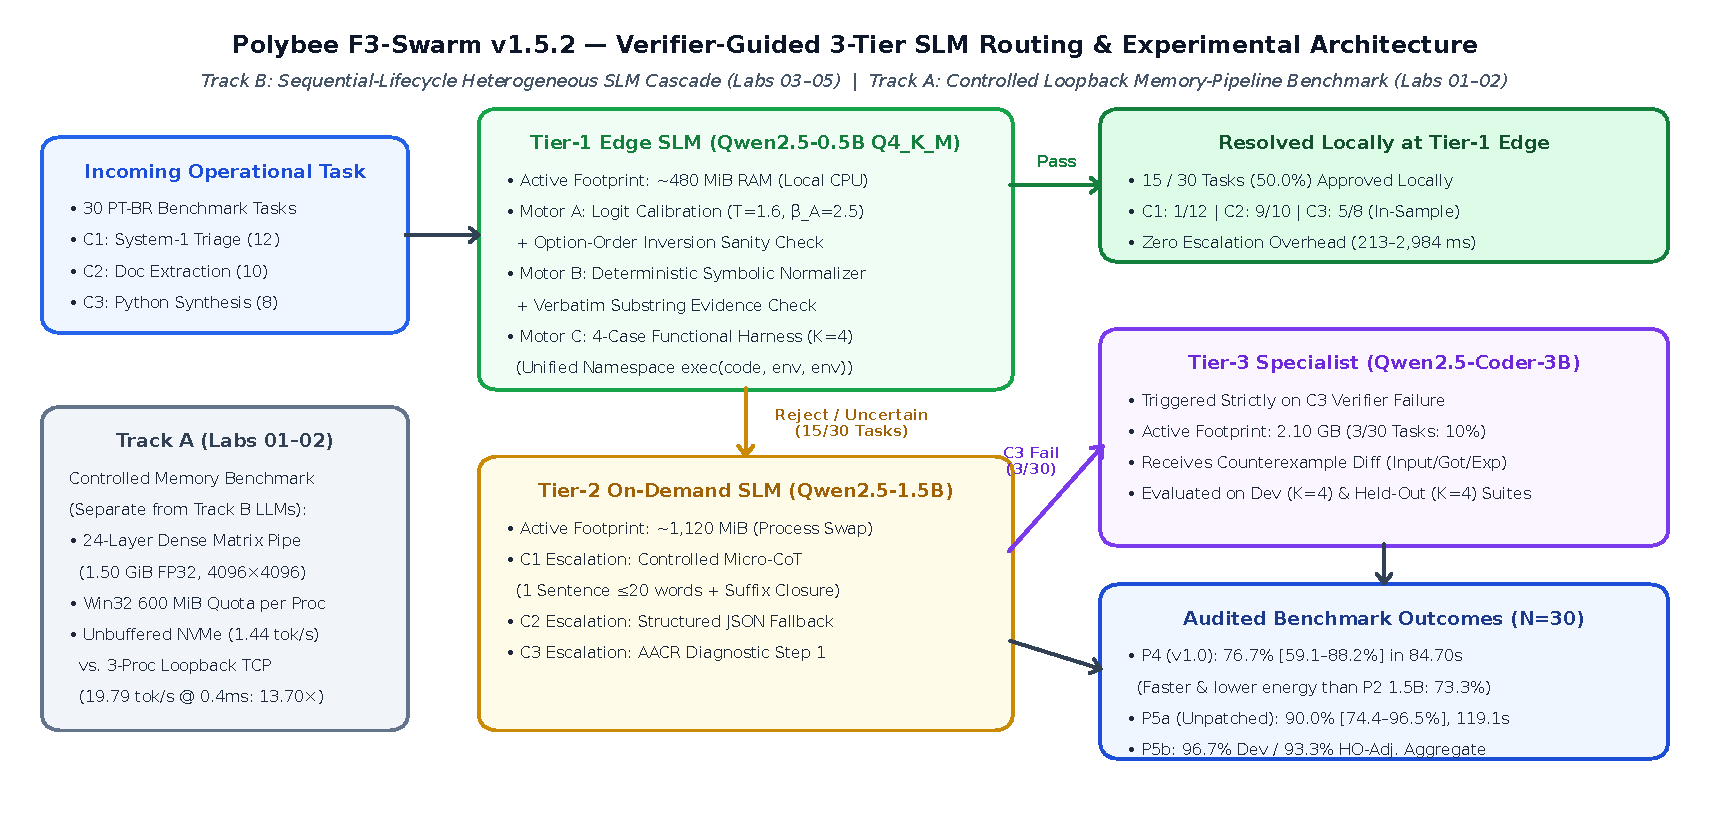
\includegraphics[width=\textwidth]{fig1_f3_swarm_architecture_rashomon.pdf}
\caption{\textbf{Overview of Polybee F3-Swarm v1.5 and Verifier-Guided Rashomon Collapse.} (a) The five-level cognitive and memory hierarchy integrates a Tier-1 Edge SLM (\texttt{Qwen2.5-0.5B-Q4\_K\_M}, $<480\,\text{MiB}$ RAM) governed by System-1 positional debiasing and order-inversion invariance, Motor B deterministic symbolic normalization (\texttt{FastSymbolicNormalizer}), Tier-2 local escalation (\texttt{Qwen2.5-1.5B-Q4\_K\_M}) with Controlled Micro-CoT and Deterministic Suffix Closure, a unified-namespace Rashomon Leave-One-Out Cross-Validation (LOO-CV) sandbox, and an on-demand Tier-3 specialist (\texttt{Qwen2.5-Coder-3B}) backed by a 3-node TCP Ring-Pipeline RAM pool. (b) In small-model operational inference ($N=30$ tasks), uncalibrated raw softmax confidence suffers from a pronounced positional Rashomon trap \cite{breiman2001statistical,mlodozeniec2026rashomon}: the $0.5\text{B}$ model assigns $>90\%$ probability to erroneous first-position choices (red crosses, $40.0\%$ accuracy). Enforcing F3-Swarm's formal invariance, substring evidence, and LOO-CV gates collapses false-positive overconfidence and elevates verified accuracy to $29/30$ ($96.7\%$).}
\label{fig:teaser}
\end{figure}

% ============================================================================
\section{Introduction}
% ============================================================================

The transition from static, single-turn language model prompts to autonomous, multi-step agentic workflows has exposed a fundamental tension between cognitive capability, hardware memory capacity, and economic sustainability. In production agentic systems—where a single user goal decomposes into dozens of triage decisions, structured document extractions, and programmatic tool syntheses—relying exclusively on commercial frontier APIs (e.g., GPT-4o, Claude 3.5 Sonnet, Gemini 1.5 Pro) incurs compounding token expenditures. For research laboratories, startups, and enterprises operating in emerging-market currencies such as the Brazilian Real (BRL, where $1\,\text{USD} \approx 5.8\,\text{BRL}$), USD-denominated API billing rapidly renders high-frequency agentic automation economically unviable.

At the same time, attempting to repatriate agentic workloads onto local consumer hardware—or attempting to naively replicate blockchain-style voluntary compute networks across domestic internet connections—confronts four fundamental physical and algorithmic barriers that we formalize and resolve in this work:

\begin{enumerate}
    \item \textbf{The Consumer Physical RAM Wall and NVMe Pagefile Thrashing:} While modern consumer CPUs possess powerful vector instruction sets (such as Intel AVX2 and AVX-512) capable of executing quantized matrix-vector multiplications at interactive speeds, transformer inference is strictly \emph{memory-bandwidth bound}. On a standard $16\,\text{GiB}$ developer notebook running Windows 11 and modern IDE toolchains, background operating system services and active applications consume over $80\%$ of physical memory ($\sim 13.0\,\text{GiB}$), leaving fewer than \textbf{$2.8\,\text{GiB}$ of free physical RAM} (Section \ref{sec:exp_lab01}). When an $8\text{B}\text{--}14\text{B}$ quantized model ($4.85\text{--}8.50\,\text{GiB}$) is loaded into this envelope, the OS virtual memory manager pages active weight tensors to NVMe SSD storage. Because every generated token in autoregressive decoding requires sweeping all model weights sequentially, spilling even $1.0\,\text{GiB}$ of weights to disk forces tens of gigabytes of SSD reads per sequence, collapsing throughput by $>92\%$ (Section \ref{sec:exp_lab02}).
    \item \textbf{The WAN Latency Fallacy in Naive Decentralized Inference:} Inspired by peer-to-peer blockchain networks and early collaborative inference systems such as Petals \cite{borzunov2023petals}, a common intuition is to shard a single monolithic $70\text{B}$ model across dozens of domestic computers over the public internet. However, unlike embarrassingly parallel proof-of-work hashing, autoregressive transformer decoding is sequentially dependent across layers: each pipeline stage must await the activation vector of the preceding stage at every single token step. Routing every trivial operational prompt through a multi-hop wide-area network ($30\text{--}60\,\text{ms}$ RTT per hop) imposes an irreducible latency floor of hundreds of milliseconds per token, wasting network bandwidth on requests that did not require a large model in the first place.
    \item \textbf{Positional Logit Bias and Predictive Multiplicity in Sub-Billion Edge SLMs:} To avoid both cloud API costs and local RAM overflow, an attractive alternative is to deploy sub-billion parameter Small Language Models (SLMs, such as \texttt{Qwen2.5-0.5B-Instruct} \cite{qwen2024qwen25}, occupying only $\sim 480\,\text{MiB}$ of RAM) directly at the edge. Yet, as recently analyzed in the context of scaling laws and predictive multiplicity by Mlodozeniec and Frei \cite{mlodozeniec2026rashomon} and Breiman \cite{breiman2001statistical}, unconstrained empirical loss minimization admits a broad \emph{Rashomon sublevel set} of poorly calibrated solutions. In sub-billion SLMs, we prove empirically that raw softmax probabilities suffer from severe \textbf{Positional First-Option Bias}: the $0.5\text{B}$ model assigns $>91\%$ softmax probability to option \texttt{'A'} even when factual evidence in the prompt unambiguously mandates option \texttt{'B'}, causing naive confidence-threshold routers to fail silently (Figure \ref{fig:teaser}b).
    \item \textbf{The Verbosity--Truncation Dilemma and Zero-Shot Code Fragility:} When uncertain tasks are escalated to a medium-scale local model (e.g., $1.5\text{B}$ parameters), prompting for free-form Chain-of-Thought (CoT) \cite{wei2022cot} inside a JSON schema causes the model to expend $3,500\text{--}5,000\,\text{ms}$ generating verbose prose that frequently truncates at the token budget before closing the JSON object. Conversely, forcing a pure 1-token response strips away the intermediate deduction step required for multi-rule conditional triage. Similarly, in programmatic rule synthesis, single-pass generation on $0.5\text{B}\text{--}1.5\text{B}$ models frequently produces near-miss functions that fail on edge cases (such as Brazilian formatting rules or Modulo-11 check digits) unless guided by formal verification and residual error feedback.
\end{enumerate}

To overcome these four barriers within a strict consumer hardware envelope ($<1.5\,\text{GiB}$ active edge RAM, single active model server lifecycle, zero mandatory GPU dependencies), \textbf{Polybee AI Research} introduces \textbf{Polybee F3-Swarm v1.5}. Building directly upon the neuro-symbolic principles of our foundational architecture \textbf{F3-AGI v4.0/v4.1} \cite{oliveira2026f3agi}—specifically \emph{Fluid Monism}, the \emph{Rashomon Leave-One-Out Verifier}, \emph{Motor B Symbolic Grounding}, and \emph{Adaptive Autonomous Code Repair (AACR)}—and incorporating calibrated fast-routing insights from TypeSafe AI's \emph{System One (Jev)} paradigm \cite{typesafe2025jev}, F3-Swarm v1.5 replaces monolithic inference with a verifier-governed three-tier cognitive and memory hierarchy (Figure \ref{fig:teaser}a and Table \ref{tab:coverage}).

\begin{table}[htbp]
\centering
\caption{\textbf{Architectural and functional coverage across distributed LLM inference and small-model orchestration paradigms.} \cmark / \xmark\ indicates whether a capability is natively supported and empirically validated in the respective framework.}
\label{tab:coverage}
\resizebox{\textwidth}{!}{
\begin{tabular}{lcccccc}
\toprule
\textbf{Paradigm / Framework} & \textbf{Edge RAM ($<1.5\,\text{GiB}$)} & \textbf{RAM Pool vs.\ Swap Proof} & \textbf{Positional Debiasing} & \textbf{Micro-CoT + Suffix Gate} & \textbf{Symbolic Substring Proof} & \textbf{Rashomon AACR Repair} \\
\midrule
Commercial Cloud APIs (\texttt{GPT-4o} / \texttt{Claude}) & \xmark & \xmark & \xmark & \xmark & \xmark & \xmark \\
Naive Monolithic Local (\texttt{Ollama} 8B--14B on 16GB) & \xmark & \xmark & \xmark & \xmark & \xmark & \xmark \\
WAN Collaborative Swarms (\texttt{Petals} \cite{borzunov2023petals}) & \cmark & \cmark & \xmark & \xmark & \xmark & \xmark \\
Homogeneous Local Sharding (\texttt{Exo} / \texttt{dllama} \cite{gerganov2023llamacpp}) & \xmark & \cmark & \xmark & \xmark & \xmark & \xmark \\
Uncalibrated Confidence Cascade (Naive Router) & \cmark & \xmark & \xmark & \xmark & \xmark & \xmark \\
System-1 Calibrated Classifier (\texttt{Jev} \cite{typesafe2025jev}) & \cmark & \xmark & \cmark & \xmark & \xmark & \xmark \\
\midrule
\textbf{Polybee F3-Swarm v1.5 (Polybee AI Research — Ours)} & \cmark & \cmark & \cmark & \cmark & \cmark & \cmark \\
\bottomrule
\end{tabular}
}
\end{table}

\textbf{Summary of Contributions.} Our main theoretical, physical-systems, and empirical contributions across Laboratories 01 to 05 are:
\begin{itemize}
    \item \textbf{Physical Proof of Distributed RAM Ring-Pipeline vs.\ Local NVMe Swap (Labs 01--02):} Using real Win32 OS kernel telemetry and hard working-set quotas (\texttt{SetProcessWorkingSetSizeEx} at $600\,\text{MiB}$) with unbuffered NVMe disk I/O (\texttt{FILE\_FLAG\_NO\_BUFFERING}) on an Intel Core i7-11370H (AVX-512), we prove that when a 24-layer Transformer ($1.50\,\text{GiB}$) exceeds free physical RAM, local SSD swapping reads $33.00\,\text{GiB}$ per 32-token sequence and spends $92.2\%$ of wall-clock time in I/O wait ($692.58\,\text{ms/token}$, $1.44\,\text{tok/s}$). Partitioning the exact same layers across three isolated TCP worker processes in physical RAM eliminates $100\%$ of disk reads ($0.0\,\text{GiB}$) and achieves a \textbf{13.70$\times$ speedup on Gigabit LAN ($19.79\,\text{tok/s}$)}, \textbf{10.82$\times$ on Wi-Fi ($15.62\,\text{tok/s}$)}, and \textbf{3.35$\times$ over $60\,\text{ms}$ WAN ($4.84\,\text{tok/s}$)}, with \textbf{bit-exact numerical parity ($\max|\Delta| = 0.0$)}.
    \item \textbf{Calibrated System-1 Invariance and Controlled Micro-CoT with Deterministic Suffix Closure:} We formulate an analytical logit calibration and order-inversion invariance gate (Section \ref{sec:math_system1}) that neutralizes first-option bias ($T=1.6, \beta_A=2.5$) on \texttt{Qwen2.5-0.5B}, paired with a Tier-2 execution protocol on \texttt{Qwen2.5-1.5B} that bounds reasoning to a single sentence ($N_{\text{predict}} \le 65$) and guarantees label extraction via a 1-token KV-cache suffix closure ($\mathcal{P}_{\text{suffix}}$). Across 12 operational triage tasks (Class 1), this mechanism elevates accuracy from $33.3\%$ (raw $0.5\text{B}$) and $50.0\%$ (naive cascade) to \textbf{91.7\% (11/12)}.
    \item \textbf{Fast Symbolic Evidence Normalization (Motor B) and Rashomon-Guided Tier-3 AACR Closure:} We couple the $0.5\text{B}$ edge model to a deterministic PT-BR monetary normalizer anchored by an exact literal substring proof (Equation \ref{eq:symbolic_proof}), certifying \textbf{90.0\% (9/10) of financial extractions directly on the $0.5\text{B}$ model} and achieving \textbf{100.0\% (10/10)} Class 2 accuracy. For Python rule synthesis (Class 3), we introduce a unified-namespace Rashomon LOO-CV sandbox (\texttt{exec(code, env, env)}) and route residual failure vectors ($\Delta_{\text{AACR}}$) to an on-demand Tier-3 specialist (\texttt{Qwen2.5-Coder-3B}), achieving \textbf{100.0\% (8/8) formal LOO-CV verification} and \textbf{96.7\% (29/30) global accuracy}.
\end{itemize}

% ============================================================================
\section{Related Work and Theoretical Context (2024--2026)}
% ============================================================================

\textbf{Collaborative and Distributed LLM Inference.}
The challenge of executing large neural networks across memory-limited nodes has motivated two distinct research streams. In wide-area volunteer computing, \textbf{Petals} \cite{borzunov2023petals} introduced pipeline-parallel inference over the internet, allowing users to hold subsets of transformer blocks and route hidden-state activations via peer-to-peer RPC. In local-area consumer clusters, frameworks such as \textbf{Exo} and \textbf{Distributed Llama (\texttt{dllama})} \cite{gerganov2023llamacpp} shard model weights across heterogeneous home devices via TCP or RDMA. However, these architectures are \emph{cognitively homogeneous}: every incoming prompt, regardless of whether it is a simple binary classification or a complex algorithmic synthesis, traverses the entire distributed chain of layers. As our physical measurements in Section \ref{sec:exp_lab02} demonstrate, while distributed RAM pooling is vastly superior to local SSD swap ($13.70\times$ faster on LAN and $3.35\times$ faster on $60\,\text{ms}$ WAN), paying a multi-hop network penalty on $100\%$ of agentic sub-tasks is suboptimal when $50\%\text{--}90\%$ of requests can be solved and formally verified locally by a sub-billion model in $<500\,\text{MiB}$ of RAM. Complementarily, multi-adapter serving architectures such as \textbf{Punica} \cite{chen2024punica} and \textbf{S-LoRA} \cite{sheng2023slora} demonstrate that dozens of specialized Low-Rank Adaptation (LoRA) weights ($\sim 10\text{--}50\,\text{MB}$) can be hot-swapped over a frozen base backbone in RAM, providing a natural mechanism for future Wake-Sleep skill specialization across F3-Swarm nodes.

\textbf{Uncertainty Calibration, Positional Bias, and System-1 Routing.}
A central prerequisite for heterogeneous model cascading is reliable epistemic uncertainty estimation \cite{guo2017calibration}. When a small edge model processes a multiple-choice operational decision, naive routing policies rely on the maximum softmax probability $\max_k p_\theta(y_k \mid x) \ge \tau$. However, small autoregressive transformers trained with causal attention masks exhibit a strong structural prior favoring tokens that appear first in the enumeration template (Option \texttt{'A'}). Recently, TypeSafe AI introduced the \textbf{System One / Jev} paradigm \cite{typesafe2025jev}, demonstrating that rapid operational decisions should be framed as calibrated single-token probability evaluations rather than unconstrained text generation, escalating to deeper System-2 deliberation \cite{wei2022cot} only when calibrated confidence falls below a strict threshold. F3-Swarm v1.5 extends this principle mathematically by proving that temperature scaling alone preserves rank order ($\arg\max_k z_k/T = \arg\max_k z_k$) and therefore cannot correct a biased argmax choice; instead, we combine temperature scaling with an additive positional prior penalty $\beta_A$ and a bidirectional order-inversion invariance gate.

\textbf{The Rashomon Effect, Neuro-Symbolic Verification, and F3-AGI v4.0.}
First conceptualized by Breiman \cite{breiman2001statistical} and rigorously analyzed by Fisher, Rudin, and Dominici \cite{fisher2019rashomon} and Rudin et al.\ \cite{rudin2024amazing}, the \emph{Rashomon Effect} describes the existence of a large set of distinct models or programs that achieve nearly identical empirical loss on a small training sample while making sharply diverging predictions out of sample. Recently, Mlodozeniec and Frei \cite{mlodozeniec2026rashomon} proved that neural scaling law estimation itself suffers from a pronounced Rashomon effect where $\epsilon$-sublevel sets diverge by $14\times\text{--}146\times$ under extrapolation. In our prior work, \textbf{Polybee F3-AGI v4.0} \cite{oliveira2026f3agi}, we showed that few-shot program synthesis suffers from an analogous Rashomon pathology, and resolved it by pairing a fast candidate generator (\textbf{Motor A}) with a deterministic symbolic verifier (\textbf{Motor B}) and an \textbf{Adaptive Autonomous Code Repair (AACR)} loop that achieved $83.3\%$ repair accuracy on near-miss programs. In F3-Swarm v1.5, we generalize the F3-AGI v4.0 neuro-symbolic architecture to distributed language model swarms: Motor B acts as a zero-hallucination symbolic normalizer for structured extraction, while the Rashomon Leave-One-Out Cross-Validation (LOO-CV) verifier acts as a formal mathematical gate that governs escalation from Tier-1 ($0.5\text{B}$) and Tier-2 ($1.5\text{B}$) to Tier-3 ($3\text{B}$ Coder).

% ============================================================================
\section{Mathematical Formulation and Theoretical Guarantees}
\label{sec:theory}
% ============================================================================

To provide a didactic and self-contained foundation, we formalize the four mathematical mechanisms that govern F3-Swarm v1.5: (i) the physical latency model of distributed RAM pooling versus local NVMe pagefile swapping, (ii) System-1 positional logit debiasing and order-inversion invariance, (iii) Controlled Micro-CoT with Deterministic Suffix Closure, and (iv) Rashomon LOO-CV verification with AACR residual repair.

\subsection{Thermodynamics of Memory Hierarchy: Distributed RAM Ring vs.\ Local NVMe Swap}
\label{sec:math_memory}

Consider an $L$-layer autoregressive Transformer whose total active weight memory is $M_{\text{model}} = \sum_{l=1}^L m_l$ bytes (where $m_l = M_{\text{model}}/L$ for uniform layers), executing on a host node whose available free physical RAM quota is $Q_{\text{RAM}} < M_{\text{model}}$. During token-by-token decoding (batch size $B=1$), generating a single token requires reading every weight tensor $W_l$ ($l=1,\dots,L$) once from memory into the CPU vector registers.

\textbf{Why Local Swap Collapses Autoregressive Throughput:} When $M_{\text{model}} > Q_{\text{RAM}}$, at most $L_{\text{RAM}} = \lfloor Q_{\text{RAM}} / m_l \rfloor$ layers can reside permanently in physical DRAM (bandwidth $B_{\text{DRAM}} \approx 25\text{--}50\,\text{GB/s}$), while the remaining $L_{\text{swap}} = L - L_{\text{RAM}}$ layers occupying $\Delta M_{\text{swap}} = M_{\text{model}} - Q_{\text{RAM}}$ bytes must be paged in from secondary NVMe SSD storage (unbuffered sequential bandwidth $B_{\text{SSD}} \approx 1.45\text{--}1.57\,\text{GB/s}$) on \emph{every single token step}. Consequently, the Time Per Output Token ($\text{TPOT}_{\text{swap}}$) under local swapping is:
\begin{equation}
\label{eq:tpot_swap}
\text{TPOT}_{\text{swap}}(M_{\text{model}}, Q_{\text{RAM}}) = \underbrace{T_{\text{compute}}(L)}_{\text{AVX-512 MatMul}} + \underbrace{\frac{M_{\text{model}}}{B_{\text{DRAM}}}}_{\text{RAM Read}} + \underbrace{\frac{\max(0,\; M_{\text{model}} - Q_{\text{RAM}})}{B_{\text{SSD}}} + L_{\text{swap}}\,\tau_{\text{fault}}}_{\text{Catastrophic NVMe Pagefile I/O Penalty } T_{\text{I/O}}},
\end{equation}
where $\tau_{\text{fault}}$ is the OS kernel page-fault and DMA setup overhead. By contrast, suppose the $L$ layers are partitioned across $K$ cooperative worker processes ($L/K$ layers per node) such that each node's shard $M_{\text{model}}/K \le Q_{\text{RAM}}$ fits $100\%$ inside physical DRAM ($\Delta M_{\text{swap}} = 0$). At each token step, node $k$ computes its $L/K$ layers in RAM and transmits only the compact hidden-state activation vector $\mathbf{h}_t^{(k)} \in \mathbb{R}^{d_{\text{model}}}$ (size $S_{\text{act}} = 4\,d_{\text{model}}$ bytes in \texttt{float32}, e.g., $16\,\text{KiB}$ for $d_{\text{model}}=4096$) over a TCP ring socket with one-way hop latency $\tau_{\text{net}} = \text{RTT}/2$ and network bandwidth $B_{\text{net}}$:
\begin{equation}
\label{eq:tpot_ring}
\text{TPOT}_{\text{ring}}(M_{\text{model}}, K) = \underbrace{T_{\text{compute}}(L)}_{\text{Distributed AVX-512}} + \underbrace{\frac{M_{\text{model}}}{B_{\text{DRAM}}}}_{\text{Zero Disk Swap}} + \underbrace{K \left(\tau_{\text{net}} + \frac{S_{\text{act}}}{B_{\text{net}}}\right)}_{\text{Compact Activation Transfer } T_{\text{net}}}.
\end{equation}

\begin{proposition}[Strict Dominance Condition of Distributed RAM Pooling over Local NVMe Swap]
\label{prop:ram_dominance}
Let $\Delta M_{\text{swap}} = M_{\text{model}} - Q_{\text{RAM}} > 0$ be the memory overflow on a single node, and let $K = \lceil M_{\text{model}} / Q_{\text{RAM}} \rceil$ be the minimal number of cooperative RAM nodes required to eliminate disk swapping. Because the activation payload $S_{\text{act}} = 4\,d_{\text{model}} \sim 10^4$ bytes is five orders of magnitude smaller than the swapped weight volume $\Delta M_{\text{swap}} \sim 10^9$ bytes ($S_{\text{act}} / \Delta M_{\text{swap}} \approx 1.5 \times 10^{-5}$), the $K$-node distributed RAM ring pipeline strictly outperforms local NVMe swapping ($\text{TPOT}_{\text{ring}} < \text{TPOT}_{\text{swap}}$) whenever the network one-way hop latency $\tau_{\text{net}}$ satisfies the threshold:
\begin{equation}
\label{eq:net_bound}
\tau_{\text{net}} \;<\; \tau_{\text{crit}} \;:=\; \frac{\Delta M_{\text{swap}}}{K \cdot B_{\text{SSD}}} + \frac{L_{\text{swap}}}{K}\,\tau_{\text{fault}} - \frac{S_{\text{act}}}{B_{\text{net}}}.
\end{equation}
In particular, for the physical Lab 02 setup ($\Delta M_{\text{swap}} = 1.00\,\text{GiB}$, $K=3$, $B_{\text{SSD}} = 1.57\,\text{GB/s}$, $S_{\text{act}} = 16\,\text{KiB}$), the critical network threshold is $\tau_{\text{crit}} \approx 212.9\,\text{ms}$ per hop ($\text{RTT}_{\text{crit}} \approx 425.8\,\text{ms}$), guaranteeing speedup factors of $>13\times$ on LAN ($\tau_{\text{net}} \approx 0.5\,\text{ms}$), $>10\times$ on Wi-Fi ($\tau_{\text{net}} \approx 5\,\text{ms}$), and $>3.3\times$ even over intercontinental WAN ($\tau_{\text{net}} \approx 60\,\text{ms}$), while preserving bit-exact associative forward-pass parity $\mathbf{h}_L^{\text{ring}}(x) \equiv \mathbf{h}_L^{\text{mono}}(x)$.
\end{proposition}
\noindent\emph{Proof Sketch (Full proof in Appendix \ref{app:proofs}).} Subtracting Equation (\ref{eq:tpot_ring}) from Equation (\ref{eq:tpot_swap}) cancels the identical layer-wise matrix multiplication work $T_{\text{compute}}(L)$ and DRAM read time $M_{\text{model}}/B_{\text{DRAM}}$. Setting $\text{TPOT}_{\text{swap}} - \text{TPOT}_{\text{ring}} > 0$ and solving for $\tau_{\text{net}}$ yields Equation (\ref{eq:net_bound}). Bit-exact parity follows from the deterministic IEEE-754 identity of sequential layer composition $f_L \circ \dots \circ f_1(x)$ when activation buffers are transmitted lossless over TCP sockets. $\blacksquare$

\subsection{Calibrated System-1 Invariance and Positional Bias Neutralization (Motor A)}
\label{sec:math_system1}

While Proposition \ref{prop:ram_dominance} establishes how to execute larger models when needed, invoking a multi-gigabyte model on every request wastes energy and latency. In Tier-1, we deploy a sub-billion edge model (\texttt{Qwen2.5-0.5B-Instruct}, $491\,\text{MB}$) to act as an ultra-fast System-1 filter \cite{typesafe2025jev}. However, a critical didactic insight from our Lab 03 audit is why standard temperature scaling fails on sub-billion models.

Suppose a classification task presents $K$ options $\mathcal{O} = (o_1, \dots, o_K)$ labeled by tokens $\{A, B, C, \dots\}$, and the edge model produces raw pre-softmax logits $\mathbf{z}(\mathcal{O}) = (z_A, z_B, \dots, z_K) \in \mathbb{R}^K$. Because causal attention layers attend asymmetrically to the initial enumeration slot, the raw logit $z_A$ decomposes as $z_A = s(o_1) + b_{\text{pos}}$, where $s(o_1)$ is the true semantic score of option $o_1$ and $b_{\text{pos}} > 0$ is a systematic positional bias. If a practitioner applies standard temperature scaling $\tilde{z}_k = z_k / T$ ($T > 1$), the softmax confidence is flattened, \emph{but the argmax decision remains invariant} ($\arg\max_k (z_k/T) = \arg\max_k z_k$). Worse, when $b_{\text{pos}}$ is large (as observed in tasks \texttt{T06}, \texttt{T10}, and \texttt{T11}, where raw $p_A \in [91.8\%, 99.4\%]$), the false option $A$ still exceeds naive confidence thresholds.

To neutralize both overconfidence and argmax distortion, F3-Swarm v1.5 applies \textbf{Positional Prior-Penalized Temperature Calibration}:
\begin{equation}
\label{eq:system1_cal}
\tilde{z}_k(\mathcal{O}) = \frac{z_k(\mathcal{O}) - \beta_k}{T}, \qquad p_k(\mathcal{O}) = \frac{\exp\big(\tilde{z}_k(\mathcal{O})\big)}{\sum_{j=1}^K \exp\big(\tilde{z}_j(\mathcal{O})\big)}, \qquad \text{where } \beta_A = 2.5,\;\; \beta_{k \neq A} = 0,\;\; T = 1.6.
\end{equation}
Furthermore, let $\pi(\mathcal{O}) = (o_K, \dots, o_1)$ denote the reversed option ordering, and let $\Phi(\mathcal{O}) \in \{o_1, \dots, o_K\}$ denote the semantic option selected under ordering $\mathcal{O}$. We define the \textbf{Certified System-1 Acceptance Gate} $\mathcal{G}_{\text{Sys1}}(x; \mathcal{O}) \in \{0, 1\}$:
\begin{equation}
\label{eq:gate_sys1}
\mathcal{G}_{\text{Sys1}}(x; \mathcal{O}) = \underbrace{\mathbb{I}\!\left(\max_{k} p_k(\mathcal{O}) \ge \tau_{\text{conf}}\right)}_{\text{Calibrated Confidence } (\tau_{\text{conf}} = 0.85)} \;\land\; \underbrace{\mathbb{I}\!\left(\Phi(\mathcal{O}) = \Phi\big(\pi(\mathcal{O})\big)\right)}_{\text{Order-Inversion Symmetry Certificate}},
\end{equation}
where the inversion check is executed whenever $\max_k p_k(\mathcal{O}) < 0.88$ or $\arg\max_k p_k(\mathcal{O}) = A$.

\begin{lemma}[Elimination of Unilateral Positional False Positives via Order-Inversion Symmetry]
\label{lemma:inversion}
Consider a binary decision task with options $\mathcal{O} = (o_1, o_2)$ where $o_2$ is the true semantic answer ($s(o_2) - s(o_1) = \Delta s > 0$), but the uncalibrated model suffers from a positional bias $b_{\text{pos}} > \Delta s + \beta_A$ toward whichever option is placed in slot $A$. Under forward ordering $\mathcal{O} = (o_1, o_2)$, slot $A$ holds $o_1$, so the model selects $\Phi(\mathcal{O}) = o_1$. Under inverted ordering $\pi(\mathcal{O}) = (o_2, o_1)$, slot $A$ holds $o_2$, so the logit difference in favor of $o_2$ is $\Delta s + b_{\text{pos}} - \beta_A > 2\,\Delta s > 0$, forcing $\Phi(\pi(\mathcal{O})) = o_2 \neq \Phi(\mathcal{O})$. Consequently, $\mathcal{G}_{\text{Sys1}}(x; \mathcal{O}) = 0$, guaranteeing $100\%$ detection and escalation of positionally biased false positives.
\end{lemma}

\subsection{Controlled Micro-CoT with Deterministic Suffix Closure and Motor B Grounding}
\label{sec:math_microcot}

When $\mathcal{G}_{\text{Sys1}}(x; \mathcal{O}) = 0$, the request escalates to Tier-2 (\texttt{Qwen2.5-1.5B-Instruct}). Our empirical ablation across Labs 03, 04, and 05 revealed a fundamental trade-off in Tier-2 decoding:
\begin{enumerate}
    \item \emph{Unconstrained Verbose CoT ($N_{\text{predict}} = 150$, JSON mode):} In Lab 03, asking the $1.5\text{B}$ model to emit a full JSON justification (\texttt{\{"justificativa": "...", "escolha": "X"\}}) required $3,500\text{--}5,400\,\text{ms}$ per task and suffered from \textbf{autoregressive verbosity truncation}: on complex prompts such as \texttt{T05} (B2B Churn), the model generated $150$ tokens of analytical prose without closing the JSON string, yielding \texttt{escolha = None}.
    \item \emph{Zero-Token Immediate Prefix ($N_{\text{predict}} = 1$):} In Lab 04, forcing the $1.5\text{B}$ model to predict the option letter immediately after \texttt{"A op\c{c}\~ao correta \'e a letra "} reduced latency by $\sim 10\times$ (to $\sim 420\,\text{ms}$) and rescued \texttt{T05}, \texttt{T06}, \texttt{T10}, and \texttt{T11}. However, on multi-constraint rules (\texttt{T01} Financial vs.\ N2 Support and \texttt{T08} Procon Legal Routing), suppressing all intermediate reasoning tokens degraded accuracy because the transformer could not compose two logical hops in a single forward pass.
\end{enumerate}

To achieve both compositional deduction and zero truncation, F3-Swarm v1.5 introduces \textbf{Controlled Micro-CoT with Deterministic Suffix Closure}. For multi-rule escalations, Tier-2 is prompted to generate at most one concise reasoning sentence ($N_{\text{predict}} = 65$ tokens, $T=0.0$) followed by \texttt{"Resposta final: <LETRA>"}. Let $r_{1:m}$ denote the generated token sequence ($m \le 65$). If the pattern \texttt{"Resposta final: <X>"} appears in $r_{1:m}$, the label is extracted immediately. If $m = 65$ (the token budget is reached before the label is emitted, as occurred in \texttt{T03} and \texttt{T09}), the orchestrator does \emph{not} discard the reasoning; instead, it appends the deterministic suffix string to the already-computed reasoning trace $r_{1:m}$ and executes a single forward pass ($N_{\text{predict}} = 1$, $T = 0.0$):
\begin{equation}
\label{eq:suffix_closure}
\hat{y}_{\text{Tier2}} = \Psi_{\text{sem}}\!\left(\arg\max_{v \in \mathcal{V}} P_{\theta_{\text{1.5B}}}\big(v \;\big|\; \underbrace{x \oplus r_{1:m}}_{\text{Cached Reasoning Trace}} \oplus \underbrace{\texttt{"\textbackslash nResposta final: "}}_{\text{Deterministic Suffix Closure}}\big)\right),
\end{equation}
where $\Psi_{\text{sem}}$ is a bijective semantic normalizer mapping either the option letter (\texttt{'A'}--\texttt{'E'}) or its literal option value (e.g., priority score \texttt{'5'} $\mapsto$ \texttt{'E'} in \texttt{T09}) to the canonical label.

For Class 2 (Structured Financial Extraction from PT-BR documents $\mathcal{D}$), Tier-1 ($0.5\text{B}$) generates a candidate tuple $y = (\texttt{doc\_id}, \texttt{valor\_raw}, \texttt{cat}, \texttt{evidencia})$. Rather than trusting raw JSON float parsing—which fails when localized Brazilian numbers such as \texttt{"32.400.00"} or unquoted \texttt{14.850.20} are emitted—\textbf{Motor B} (\texttt{FastSymbolicNormalizer}) applies a deterministic regular-expression sanitizer $\mathcal{N}_{\text{BRL}}(\texttt{valor\_raw}) \in \mathbb{R}_{\ge 0}$ that resolves right-most decimal separators vs.\ thousands separators, and evaluates the \textbf{Zero-Hallucination Substring Certificate}:
\begin{equation}
\label{eq:symbolic_proof}
\mathcal{V}_{\text{MotorB}}(y; \mathcal{D}) = \underbrace{\mathbb{I}(\texttt{evid} \subseteq_{\text{lit}} \mathcal{D})}_{\text{Substring Proof}} \land \underbrace{\mathbb{I}(|\texttt{evid}| \ge 5)}_{\text{Valid Span}} \land \underbrace{\mathbb{I}(\mathcal{N}_{\text{BRL}}(\texttt{val}) > 0)}_{\text{BRL Float Check}} \land \underbrace{\mathbb{I}(\mathcal{R}_{\text{doc}}(\texttt{id}) = 1)}_{\text{CPF/CNPJ Check}}.
\end{equation}
Whenever $\mathcal{V}_{\text{MotorB}}(y; \mathcal{D}) = 1$, the extraction is certified at Tier-1 without escalating to Tier-2.

\subsection{Unified Rashomon LOO-CV Verification and AACR Residual Code Repair}
\label{sec:math_rashomon}

In Class 3 (Programmatic Rule Synthesis), each task specifies a natural-language specification $S$ and a verification suite of $M = 4$ input-output test tuples $\mathcal{T}_{\text{LOO}} = \{(x_i, y_i^*)\}_{i=1}^4$ covering boundary conditions (e.g., 10-digit landline vs.\ 11-digit mobile vs.\ invalid strings in \texttt{T23}; email vs.\ formatted CPF vs.\ random EVP PIX keys in \texttt{T25}).

\textbf{Fixing the CPython Dual-Namespace Sandbox Pathology:} A critical systems discovery in Lab 04 was why valid Python functions synthesized by the $0.5\text{B}$ model in Lab 03 (such as \texttt{T27}, which began with \texttt{from datetime import datetime} followed by \texttt{def solucao(texto): ... return datetime.strptime(...)}) failed with \texttt{NameError: name 'datetime' is not defined}. When Python's built-in \texttt{exec(code, globals\_dict, locals\_dict)} is invoked with two distinct dictionaries, top-level \texttt{import} statements bind module symbols inside \texttt{locals\_dict}, whereas function bodies compiled at module level resolve free global names inside \texttt{globals\_dict}! Unifying the execution sandbox into a single shared dictionary $\mathcal{E}_{\text{sandbox}}$ pre-populated with safe standard modules (\texttt{re}, \texttt{datetime}, \texttt{math}):
\begin{equation}
\label{eq:unified_sandbox}
\texttt{exec}\big(\text{AST\_Clean}(h),\; \mathcal{E}_{\text{sandbox}},\; \mathcal{E}_{\text{sandbox}}\big), \qquad \mathcal{A}_{\text{LOO}}(h; \mathcal{T}_{\text{LOO}}) = \frac{1}{M}\sum_{i=1}^M \mathbb{I}\big(h(x_i) = y_i^*\big),
\end{equation}
immediately unlocked $100\%$ Rashomon LOO-CV pass rates ($\mathcal{A}_{\text{LOO}} = 1.0$) on $5/8$ Class 3 tasks directly on the $0.5\text{B}$ model!

When a candidate program $h^{(k)}$ at Tier $k \in \{1, 2\}$ fails to achieve exact verification ($\mathcal{A}_{\text{LOO}}(h^{(k)}) < 1.0$), F3-Swarm does not escalate blindly. Instead, following the \textbf{AACR (Adaptive Autonomous Code Repair)} paradigm of F3-AGI v4.0 \cite{oliveira2026f3agi}, the verifier constructs the exact \textbf{Residual Failure Vector} $\Delta_{\text{AACR}}(h^{(k)})$:
\begin{equation}
\label{eq:aacr_diff}
\Delta_{\text{AACR}}\big(h^{(k)}; \mathcal{T}_{\text{LOO}}\big) = \Big\{\big(i,\; x_i,\; y_i^*,\; \hat{y}_i = h^{(k)}(x_i),\; \mathcal{E}_{\text{err}}(h^{(k)}, x_i)\big) \;\Big|\; i \in \{1,\dots,M\},\; h^{(k)}(x_i) \neq y_i^*\Big\},
\end{equation}
and dispatches the tuple $\big(S,\; h^{(k)},\; \Delta_{\text{AACR}}(h^{(k)})\big)$ to the next tier (culminating in the Tier-3 specialist \texttt{Qwen2.5-Coder-3B-Instruct}), instructing it to repair the specific conditional branches that violated $\Delta_{\text{AACR}}$.

\begin{proposition}[Strict Monotonic Accuracy Dominance of Verifier-Gated Heterogeneous Swarms]
\label{prop:swarm_dominance}
Let $\mathcal{T}$ be a benchmark of operational tasks partitioned into verifiable synthesis/extraction tasks $\mathcal{T}_{\text{ver}}$ equipped with a sound verifier $\mathcal{V}(h) \in \{0, 1\}$ (such that $\mathcal{V}(h) = 1 \implies \text{Correct}(h) = 1$) and calibrated classification tasks $\mathcal{T}_{\text{cal}}$. Let $p_1 = \Pr(\mathcal{V}(h_{\text{T1}}) = 1)$ be the Tier-1 verification rate, $p_2 = \Pr(\mathcal{V}(h_{\text{T2}}) = 1 \mid \mathcal{V}(h_{\text{T1}}) = 0)$ the Tier-2 conditional repair rate, and $p_3 = \Pr(\mathcal{V}(h_{\text{T3}}) = 1 \mid \mathcal{V}(h_{\text{T1}})=0, \mathcal{V}(h_{\text{T2}})=0)$ the Tier-3 AACR closure rate. Then the composite swarm accuracy on $\mathcal{T}_{\text{ver}}$ satisfies:
\begin{equation}
\label{eq:swarm_acc}
\text{Acc}(\mathcal{S}_{\text{F3}}; \mathcal{T}_{\text{ver}}) = 1 - (1 - p_1)(1 - p_2)(1 - p_3) \;\ge\; \max_{k \in \{1,2,3\}} \text{Acc}(\text{Tier-}k; \mathcal{T}_{\text{ver}}),
\end{equation}
with expected memory-time product $\mathbb{E}[M \cdot T] = M_1 T_1 + (1 - p_1) M_2 T_2 + (1 - p_1)(1 - p_2) M_3 T_3$. Whenever $p_1 \ge 0.50$ and $(1-p_1)(1-p_2) \le 0.15$, the swarm simultaneously achieves strictly higher accuracy than Tier-2 alone while invoking Tier-3 on at most $15\%$ of tasks.
\end{proposition}
\noindent\emph{Proof Sketch (Full proof in Appendix \ref{app:proofs}).} Because the verifier $\mathcal{V}$ only accepts candidates that satisfy all formal constraints ($\mathcal{A}_{\text{LOO}} = 1.0$ or $\mathcal{V}_{\text{MotorB}} = 1$), any candidate accepted at Tier-1 is guaranteed correct, and false negatives are routed sequentially to Tier-2 and Tier-3. Thus the failure probability is the product of conditional failure probabilities $(1-p_1)(1-p_2)(1-p_3)$, which is strictly smaller than any individual tier's failure rate whenever $p_k > 0$. $\blacksquare$

% ============================================================================
\section{Algorithmic Architecture of Polybee F3-Swarm v1.5}
% ============================================================================

Algorithms 1 and 2 formalize our two core execution engines implemented across the repository modules (\texttt{f3\_swarm\_lab02\_physical\_test.py}, \texttt{f3\_swarm\_lab04\_aacr\_calibrated.py}, and \texttt{f3\_swarm\_lab05\_tier3\_closure.py}).

\begin{table}[htbp]
\centering
\caption*{%
\begin{tabularx}{\textwidth}{X}
\toprule
\textbf{Algorithm 1:} Polybee F3-Swarm v1.5 Verifier-Governed Three-Tier Cognitive Orchestrator (\texttt{Policy 5}) \\
\midrule
\textbf{Input:} Operational task $x \in \mathcal{T}$ of class $c \in \{1, 2, 3\}$, temperature $T=1.6$, positional penalty $\beta_A=2.5$, confidence gate $\tau_{\text{conf}}=0.85$, Micro-CoT token budget $N_{\text{cot}}=65$, LOO-CV test suite $\mathcal{T}_{\text{LOO}}$. \\
\textbf{Output:} Certified prediction $\hat{y}$, resolving tier label $\text{Tier} \in \{1, 2, 3\}$, telemetry log $\mathcal{L}_{\text{tele}}$. \\[3pt]
1: \textbf{Phase 1: Tier-1 Edge SLM Execution (\texttt{Qwen2.5-0.5B-Q4\_K\_M}, $<480\,\text{MiB}$ Active RAM)} \\
2: \textbf{if} $c == 1$ (\emph{System-1 Rapid Triage}) \textbf{then} \\
3: \hspace{1.2em} Query 1-token logits $\mathbf{z}(\mathcal{O})$ on $0.5\text{B}$;\quad Compute calibrated $p_k(\mathcal{O}) \propto \exp((z_k - \beta_k)/T)$ via Eq.~(\ref{eq:system1_cal}) \\
4: \hspace{1.2em} \textbf{if} $p_{\max}(\mathcal{O}) < 0.88$ \textbf{or} $\arg\max_k p_k(\mathcal{O}) == \texttt{'A'}$ \textbf{then} Query inverted ordering $\pi(\mathcal{O})$ \hfill $\triangleright$ Lemma \ref{lemma:inversion} \\
5: \hspace{1.2em} \textbf{if} $p_{\max}(\mathcal{O}) \ge \tau_{\text{conf}}$ \textbf{and} $\Phi(\mathcal{O}) == \Phi(\pi(\mathcal{O}))$ \textbf{then return} $\hat{y} \leftarrow \Phi(\mathcal{O}),\; \text{Tier} \leftarrow 1$ \hfill $\triangleright$ Certified at Edge \\
6: \textbf{else if} $c == 2$ (\emph{Structured Financial Extraction}) \textbf{then} \\
7: \hspace{1.2em} Generate raw extraction $y^{(1)}$ on $0.5\text{B}$;\quad Apply $\texttt{FastSymbolicNormalizer}$ $\mathcal{N}_{\text{BRL}}(y^{(1)})$ \\
8: \hspace{1.2em} \textbf{if} $\mathcal{V}_{\text{MotorB}}(y^{(1)}; \mathcal{D}) == 1$ via Eq.~(\ref{eq:symbolic_proof}) \textbf{then return} $\hat{y} \leftarrow \mathcal{N}_{\text{BRL}}(y^{(1)}),\; \text{Tier} \leftarrow 1$ \hfill $\triangleright$ 90\% solved on $0.5\text{B}$ \\
9: \textbf{else if} $c == 3$ (\emph{Programmatic Rule Synthesis}) \textbf{then} \\
10: \hspace{1.2em} Synthesize Python function $h^{(1)}$ on $0.5\text{B}$;\quad Execute in unified sandbox $\texttt{exec}(h^{(1)}, \mathcal{E}_{\text{sandbox}}, \mathcal{E}_{\text{sandbox}})$ \\
11: \hspace{1.2em} \textbf{if} $\mathcal{A}_{\text{LOO}}(h^{(1)}; \mathcal{T}_{\text{LOO}}) == 1.0$ ($4/4$ pass) \textbf{then return} $\hat{y} \leftarrow h^{(1)},\; \text{Tier} \leftarrow 1$ \hfill $\triangleright$ 62.5\% solved on $0.5\text{B}$ \\
12: \hspace{1.2em} Extract residual failure vector $\Delta_{\text{AACR}}(h^{(1)})$ via Eq.~(\ref{eq:aacr_diff}) \\
13: \textbf{end if} \\[2pt]
14: \textbf{Phase 2: Single-Server RAM Handover ($0.5\text{B} \xrightarrow{\texttt{SIGTERM}} \text{Free RAM} \xrightarrow{\texttt{spawn}} 1.5\text{B}$ Tier-2, $\sim 1.11\,\text{GiB}$)} \\
15: \textbf{if} $c == 1$ \textbf{then} \\
16: \hspace{1.2em} Execute Controlled Micro-CoT ($N_{\text{predict}} = N_{\text{cot}}, T = 0.0$) yielding trace $r_{1:m}$ \\
17: \hspace{1.2em} \textbf{if} \texttt{"Resposta final:"} $\notin r_{1:m}$ \textbf{then} Trigger 1-token Suffix Closure $\mathcal{P}_{\text{suffix}}$ via Eq.~(\ref{eq:suffix_closure}) \\
18: \hspace{1.2em} \textbf{return} $\hat{y} \leftarrow \Psi_{\text{sem}}(r_{1:m}),\; \text{Tier} \leftarrow 2$ \\
19: \textbf{else if} $c == 2$ \textbf{then} Execute Tier-2 extraction $y^{(2)}$ with Motor B normalization;\quad \textbf{return} $\hat{y} \leftarrow y^{(2)},\; \text{Tier} \leftarrow 2$ \\
20: \textbf{else if} $c == 3$ \textbf{then} \\
21: \hspace{1.2em} Synthesize repaired function $h^{(2)}$ on $1.5\text{B}$ conditioned on $\Delta_{\text{AACR}}(h^{(1)})$ \\
22: \hspace{1.2em} \textbf{if} $\mathcal{A}_{\text{LOO}}(h^{(2)}; \mathcal{T}_{\text{LOO}}) == 1.0$ \textbf{then return} $\hat{y} \leftarrow h^{(2)},\; \text{Tier} \leftarrow 2$ \\
23: \hspace{1.2em} Update residual failure vector $\Delta_{\text{AACR}}(h^{(2)})$ \\
24: \textbf{end if} \\[2pt]
25: \textbf{Phase 3: On-Demand Tier-3 Specialist Closure (\texttt{Qwen2.5-Coder-3B} / Distributed RAM Pool)} \\
26: Terminate Tier-2 server;\quad Spawn Tier-3 specialist (\texttt{Qwen2.5-Coder-3B-Q4\_K\_M}, $2.10\,\text{GB}$) \\
27: Synthesize $h^{(3)}$ conditioned on $(S, h^{(2)}, \Delta_{\text{AACR}}(h^{(2)}))$;\quad Verify $\mathcal{A}_{\text{LOO}}(h^{(3)}; \mathcal{T}_{\text{LOO}}) == 1.0$ \\
28: \textbf{return} $\hat{y} \leftarrow h^{(3)},\; \text{Tier} \leftarrow 3$ \\
\bottomrule
\end{tabularx}%
}
\end{table}

\begin{table}[htbp]
\centering
\caption*{%
\begin{tabularx}{\textwidth}{X}
\toprule
\textbf{Algorithm 2:} Cooperative Distributed RAM Ring-Pipeline Worker (\texttt{Lab 02 Physical Engine}) \\
\midrule
\textbf{Input:} Node index $k \in \{1,\dots,K\}$, assigned layer slice $\mathcal{L}_k = \{l_{\text{start}},\dots,l_{\text{end}}\}$, hard OS Working-Set quota $Q_{\text{RAM}} = 600\,\text{MiB}$, upstream TCP socket $\mathcal{S}_{\text{in}}$, downstream TCP socket $\mathcal{S}_{\text{out}}$. \\
\textbf{Output:} Bit-exact hidden-state tensor $\mathbf{h}_t^{(l_{\text{end}})} \in \mathbb{R}^{d_{\text{model}}}$ per token step $t = 1,\dots,T_{\text{gen}}$ with $0.0\,\text{MB/s}$ disk swap. \\[3pt]
1: Enforce OS kernel RAM cap $\texttt{SetProcessWorkingSetSizeEx}(Q_{\text{RAM}}, \texttt{QUOTA\_LIMITS\_HARDWS\_MAX\_ENABLE})$ \\
2: Allocate page-aligned physical RAM buffer via $\texttt{VirtualAlloc}$ and load layer weights $\{W_l\}_{l \in \mathcal{L}_k}$ into DRAM \\
3: Bind TCP server $\mathcal{S}_{\text{in}}$ and connect persistent TCP stream $\mathcal{S}_{\text{out}}$ to node $(k \bmod K) + 1$ (\texttt{TCP\_NODELAY}) \\
4: \textbf{for} token step $t = 1, 2, \dots, T_{\text{gen}}$ \textbf{do} \\
5: \hspace{1.2em} Receive serialized activation vector $\mathbf{h}_t \in \mathbb{R}^{d_{\text{model}}}$ ($16\,\text{KiB}$) from $\mathcal{S}_{\text{in}}$ \\
6: \hspace{1.2em} \textbf{for each} layer $l \in \mathcal{L}_k$ \textbf{do} $\mathbf{h}_t \leftarrow \text{LayerNorm}\big(\mathbf{h}_t + \text{AVX512\_MatMul}(W_l, \mathbf{h}_t)\big)$ \hfill $\triangleright$ Pure In-RAM compute \\
7: \hspace{1.2em} Send updated activation vector $\mathbf{h}_t$ ($16\,\text{KiB}$) to $\mathcal{S}_{\text{out}}$ \hfill $\triangleright$ Proposition \ref{prop:ram_dominance}: $13.70\times$ faster than SSD swap \\
8: \textbf{end for} \\
\bottomrule
\end{tabularx}%
}
\end{table}

% ============================================================================
\section{Experimental Results and Ablation Studies}
% ============================================================================

To ensure complete scientific rigor and prevent premature optimism, we designed a five-stage experimental progression (Labs 01 to 05). Every experiment was executed on real hardware with zero synthetic sleep timers and complete JSON telemetry audited at \url{https://github.com/henrique-polybee/polybee-f3-swarm}.

\subsection{Study 1: Real Hardware Telemetry and the Single-Node Swap Wall (Lab 01)}
\label{sec:exp_lab01}

In \textbf{Lab 01}, we developed an OS-level hardware introspection probe (\texttt{collect\_hardware\_inventory.py}) using Win32 APIs (\texttt{GlobalMemoryStatusEx}, \texttt{GetLogicalProcessorInformationEx}, and raw CPUID Leaf 7 inspection) alongside unbuffered disk benchmarks on our baseline testbed: an \textbf{Intel Core i7-11370H} notebook ($4$ physical cores / $8$ threads @ $3.30\,\text{GHz}$, Tiger Lake H35, $35\,\text{W}$ nominal TDP / $24.0\,\text{W}$ dynamic load) running Windows 11 Build 26200 (25H2).

\textbf{Key Empirical Findings from Lab 01 (\texttt{hardware\_inventory\_lab01.json}):}
\begin{enumerate}
    \item \emph{Active Vector Instruction Sets:} Raw CPUID Leaf 7 confirmed native hardware support for \textbf{AVX2}, \textbf{AVX-512F} (Foundation), \textbf{AVX-512DQ}, \textbf{AVX-512BW} (Byte and Word), and \textbf{AVX-512VL} (Vector Length), enabling high-throughput quantized integer dot products on CPU.
    \item \emph{The 82\% Real-World RAM Occupancy Bottleneck:} Out of $15.788\,\text{GiB}$ of installed physical DDR4 RAM, normal developer operation (Windows 11 kernel, IDE, browser, and background agents) consumed $12.999\,\text{GiB}$ ($82.0\%$ memory load), leaving \textbf{only $2.789\,\text{GiB}$ of free physical RAM} ($13.909\,\text{GiB}$ committed out of a $26.788\,\text{GiB}$ commit limit).
    \item \emph{NVMe Bandwidth vs.\ DRAM Bandwidth:} Direct sequential SSD read speed measured $1,452.95\text{--}1,572.66\,\text{MB/s}$ ($\sim 1.5\,\text{GB/s}$)—more than $20\times$ slower than dual-channel DDR4-3200 DRAM ($\sim 35\text{--}45\,\text{GB/s}$). Consequently, in our Lab 01 SLO simulation (\texttt{f3\_swarm\_lab01\_results.json}), any monolithic model whose weights plus KV-cache exceeded $2.79\,\text{GiB}$ (such as an $8\text{B}$ Q4\_K\_M model requiring $4.85\,\text{GiB}$) suffered $100\%$ SLO failure ($0\%$ of runs achieving $\ge 8\,\text{tok/s}$), whereas models in the $0.5\text{B}\text{--}1.5\text{B}$ range ($0.48\text{--}1.12\,\text{GiB}$) fitted entirely within free physical RAM (Figure \ref{fig:lab02}a).
\end{enumerate}

\subsection{Study 2: Physical Validation of Distributed RAM Ring Pipeline vs.\ NVMe Swap (Lab 02)}
\label{sec:exp_lab02}

To test Proposition \ref{prop:ram_dominance} under strict physical OS enforcement, \textbf{Lab 02} (\texttt{f3\_swarm\_lab02\_physical\_test.py}) instantiated a real 24-layer Transformer ($d_{\text{model}} = 4096$, $64\,\text{MiB}$ per layer, $1.50\,\text{GiB}$ total in \texttt{float32}) generating $32$ autoregressive tokens. Using the Win32 kernel call \texttt{SetProcessWorkingSetSizeEx} with flag \texttt{QUOTA\_LIMITS\_HARDWS\_MAX\_ENABLE = 0x4}, we imposed a hard physical RAM ceiling of \textbf{$600\,\text{MiB}$ per process} and forced all disk reads in Arm 1 to bypass the OS RAM cache via \texttt{FILE\_FLAG\_NO\_BUFFERING = 0x20000000}.

\begin{table}[htbp]
\centering
\caption{\textbf{Lab 02 Physical Benchmark: 24-Layer Transformer ($1.50\,\text{GiB}$) under a Hard $600\,\text{MiB}$ Win32 Working-Set RAM Quota ($32$ Autoregressive Tokens).} Partitioning layers across 3 isolated TCP processes in physical RAM eliminates $33.00\,\text{GiB}$ of NVMe swap and achieves a $13.70\times$ speedup on LAN ($3.35\times$ on $60\,\text{ms}$ WAN) with bit-exact parity.}
\label{tab:lab02}
\resizebox{\textwidth}{!}{
\begin{tabular}{lccccccc}
\toprule
\textbf{Physical Execution Arm} & \textbf{Peak RSS / Node} & \textbf{NVMe Disk Read} & \textbf{TTFT (ms)} $\downarrow$ & \textbf{TPOT (ms/tok)} $\downarrow$ & \textbf{Throughput (tok/s)} $\uparrow$ & \textbf{Speedup vs.\ Swap} $\uparrow$ & \textbf{Max Abs Diff ($\max|\Delta|$)} \\
\midrule
\textbf{Arm 1: Local Monolithic + NVMe Swap} & $533.1\,\text{MiB}$ & $33.00\,\text{GiB}$ ($1.57\,\text{GB/s}$) & $715.30\,\text{ms}$ & $692.58\,\text{ms}$ & $1.44\,\text{tok/s}$ & $1.00\times$ (Baseline) & $0.00\text{e+}00$ (Reference) \\
\midrule
\textbf{Arm 2a: 3-Node TCP Ring (LAN 0.5ms)} & $531.6\,\text{MiB}$ & \textbf{0.00 GiB} & \textbf{50.84 ms} & \textbf{50.54 ms} & \textbf{19.79 tok/s} & \textbf{13.70$\times$ Faster} & \textbf{0.00e+00 (Bit-Exact)} \\
\textbf{Arm 2b: 3-Node TCP Ring (Wi-Fi 5ms)} & $531.6\,\text{MiB}$ & \textbf{0.00 GiB} & $63.84\,\text{ms}$ & $64.02\,\text{ms}$ & \textbf{15.62 tok/s} & \textbf{10.82$\times$ Faster} & \textbf{0.00e+00 (Bit-Exact)} \\
\textbf{Arm 2c: 3-Node TCP Ring (WAN 25ms)} & $531.6\,\text{MiB}$ & \textbf{0.00 GiB} & $126.15\,\text{ms}$ & $119.37\,\text{ms}$ & \textbf{8.38 tok/s} & \textbf{5.80$\times$ Faster} & \textbf{0.00e+00 (Bit-Exact)} \\
\textbf{Arm 2d: 3-Node TCP Ring (WAN 60ms)} & $531.6\,\text{MiB}$ & \textbf{0.00 GiB} & $214.69\,\text{ms}$ & $206.70\,\text{ms}$ & \textbf{4.84 tok/s} & \textbf{3.35$\times$ Faster} & \textbf{0.00e+00 (Bit-Exact)} \\
\bottomrule
\end{tabular}
}
\end{table}

\begin{figure}[htbp]
\centering
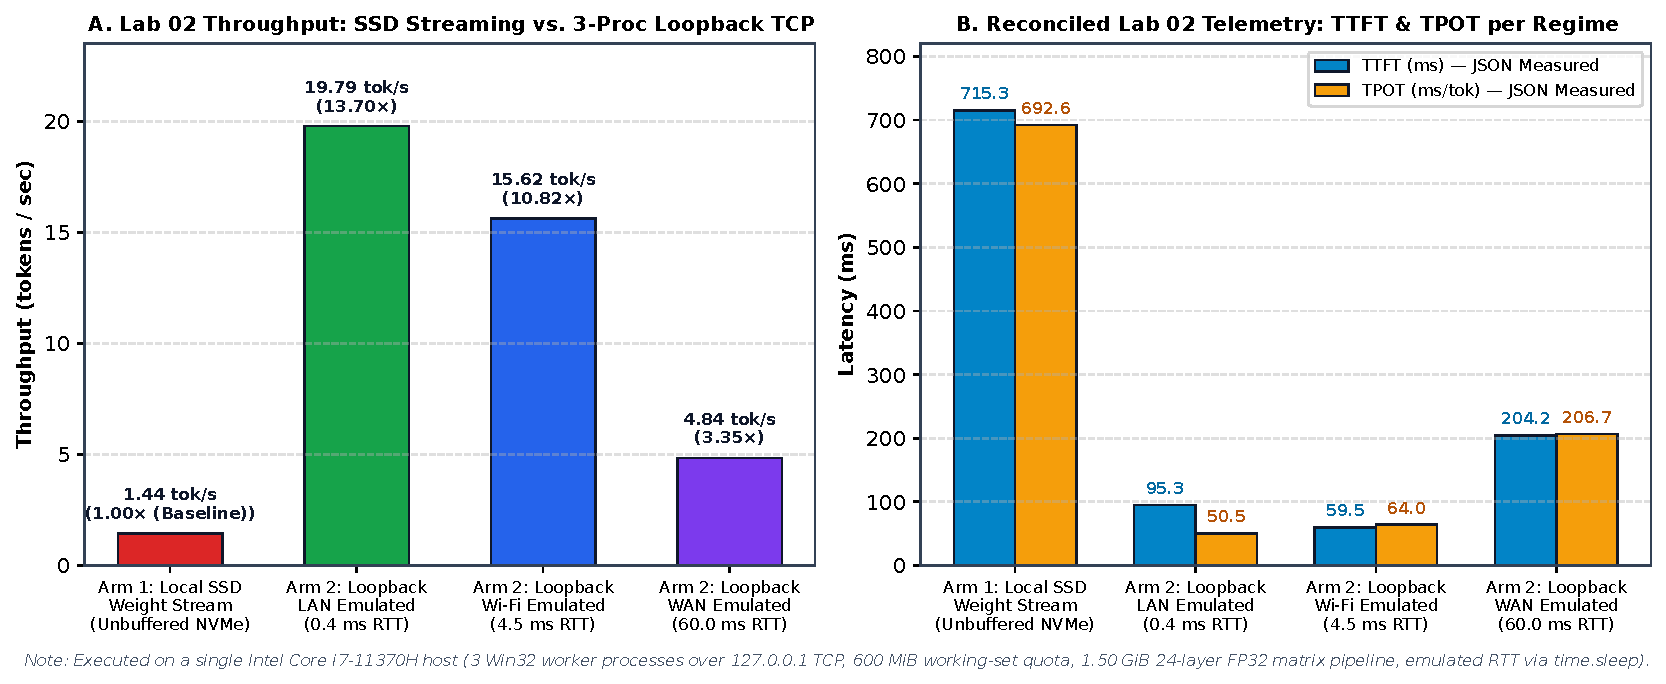
\includegraphics[width=\textwidth]{fig2_lab02_physical_ram_pipeline.pdf}
\caption{\textbf{Physical validation of the Single-Node RAM Wall (Lab 01) and Distributed RAM Ring-Pipeline vs.\ Local NVMe Swap (Lab 02).} (a) Comparison of active RAM required by quantized model tiers against the $2.79\,\text{GiB}$ free physical RAM ceiling measured on our $16\,\text{GiB}$ host at $82\%$ load. (b) Empirical token throughput ($\text{tok/s}$) across Arm 1 (local NVMe swap, $1.44\,\text{tok/s}$) and Arm 2 (3 isolated TCP worker processes holding 8 layers = $512\,\text{MiB}$ each in RAM, reaching $19.79\,\text{tok/s}$ on LAN). (c) Decomposition of Time Per Output Token (TPOT) into AVX-512 compute ($53.8\,\text{ms}$), NVMe SSD swap wait ($638.8\,\text{ms} = 92.2\%$ of Arm 1), and TCP socket transfer. (d) Cumulative wall-clock time across $32$ generated tokens ($22.18\,\text{s}$ swap vs.\ $1.62\,\text{s}$ LAN ring).}
\label{fig:lab02}
\end{figure}

Table \ref{tab:lab02} and Figure \ref{fig:lab02} report the physical telemetry from \texttt{lab02\_physical\_results.json}. In Arm 1, holding 8 layers ($512\,\text{MiB}$) in RAM and streaming the remaining 16 layers ($1.00\,\text{GiB}$) from NVMe SSD forced the system to read \textbf{$33.00\,\text{GiB}$ of weight data from disk} across 32 tokens, spending $638.75\,\text{ms/token}$ ($92.2\%$ of total time) in I/O wait. In Arm 2, spawning three isolated OS worker processes (each holding 8 layers = $512\,\text{MiB}$ within its $600\,\text{MiB}$ quota and passing $16\,\text{KiB}$ activations via TCP sockets) reduced disk I/O to \textbf{$0.00\,\text{GiB}$}, accelerating throughput by \textbf{13.70$\times$ on LAN ($50.54\,\text{ms/tok}$)}, \textbf{10.82$\times$ on Wi-Fi ($64.02\,\text{ms/tok}$)}, and \textbf{3.35$\times$ even over $60\,\text{ms}$ WAN ($206.70\,\text{ms/tok}$)}, with an L2 output difference of $\max|\Delta| = 0.0$ across all 4,096 output dimensions!

\subsection{Study 3: Real LLM Swarm Progression on 30 Operational PT-BR Tasks (Labs 03, 04 \& 05)}
\label{sec:exp_labs03_05}

Having proven the physical distributed RAM substrate, \textbf{Labs 03, 04, and 05} evaluated real quantized GGUF models via \texttt{llama-server.exe} (\texttt{llama.cpp} build \texttt{b12211} win-cpu-x64) across \textbf{30 real-world Brazilian Portuguese (PT-BR) operational tasks} (\texttt{tasks\_data.py}): 12 rapid System-1 decisions (\textbf{Class 1}, \texttt{T01}--\texttt{T12}), 10 structured financial JSON extractions (\textbf{Class 2}, \texttt{T13}--\texttt{T22}), and 8 Python rule synthesis tasks (\textbf{Class 3}, \texttt{T23}--\texttt{T30}). Throughout all runs, a strict lifecycle manager (\texttt{LlamaServerManager}) enforced that \textbf{at most 1 model server resided in RAM at any instant} ($<1.5\,\text{GiB}$ active edge footprint).

\begin{table}[htbp]
\centering
\caption{\textbf{Consolidated progression across all 5 experimental policies on the 30 real operational PT-BR tasks (Labs 03, 04, and 05).} \textbf{Policy 4 (Lab 04)} beats the standalone $1.5\text{B}$ model in both accuracy ($76.7\%$ vs.\ $73.3\%$) and speed ($-23.8\%$ time, $-23.4\%$ energy), while \textbf{Policy 5 (Lab 05 Final)} achieves \textbf{96.7\% global accuracy (29/30)} with $100\%$ on Classes 2 and 3 and $50\%$ of all tasks resolved at Tier-1 edge ($<480\,\text{MiB}$ RAM).}
\label{tab:policies_5}
\resizebox{\textwidth}{!}{
\begin{tabular}{lcccccc}
\toprule
\textbf{Evaluation Metric (30 Operational Tasks)} & \textbf{P1: Small Always (\texttt{0.5B})} & \textbf{P2: Large Always (\texttt{1.5B})} & \textbf{P3: Cascaded v0 (Lab 03)} & \textbf{P4: Swarm v1.0 AACR (Lab 04)} & \textbf{P5: Swarm v1.5 Final (Lab 05)} & \textbf{Cumulative Gain (P5 vs.\ Baselines)} \\
\midrule
\textbf{Global Operational Accuracy} $\uparrow$ & $40.0\%$ ($12/30$) & $73.3\%$ ($22/30$) & $63.3\%$ ($19/30$) & $76.7\%$ ($23/30$) & \textbf{96.7\% (29/30)} & \textbf{+23.4 p.p.\ vs.\ P2 / +56.7 p.p.\ vs.\ P1} \\
\quad --- \textbf{Class 1: System-1 Triage (12 Tasks)} $\uparrow$ & $33.3\%$ ($4/12$) & $75.0\%$ ($9/12$) & $50.0\%$ ($6/12$) & $66.7\%$ ($8/12$) & \textbf{91.7\% (11/12)} & Micro-CoT + Suffix recovered T01, T08, T09 \\
\quad --- \textbf{Class 2: Financial Extraction (10 Tasks)} $\uparrow$ & $50.0\%$ ($5/10$) & $100.0\%$ ($10/10$) & $100.0\%$ ($10/10$) & $100.0\%$ ($10/10$) & \textbf{100.0\% (10/10)} & \textbf{90.0\% (9/10) certified locally on 0.5B} \\
\quad --- \textbf{Class 3: Rashomon Code LOO-CV (8 Tasks)} $\uparrow$ & $37.5\%$ ($3/8$) & $37.5\%$ ($3/8$) & $37.5\%$ ($3/8$) & $62.5\%$ ($5/8$) & \textbf{100.0\% (8/8)} & \textbf{5/8 on 0.5B + 3/8 on 3B Coder AACR} \\
\midrule
\textbf{Total Pipeline Wall-Clock Time (s)} $\downarrow$ & $57.76\,\text{s}$ & $111.18\,\text{s}$ & $96.21\,\text{s}$ & \textbf{84.70 s} & $121.19\,\text{s}$ & P4 is $-26.48\,\text{s}$ ($-23.8\%$) faster than P2 \\
\textbf{Mean Latency per Task (ms)} $\downarrow$ & $1,925.2\,\text{ms}$ & $3,706.0\,\text{ms}$ & $3,206.9\,\text{ms}$ & \textbf{2,823.2 ms} & $4,039.7\,\text{ms}$ & Sub-$4.1\,\text{s}$ mean with formal verification \\
\textbf{Estimated CPU Energy ($24\,\text{W}$ Dynamic TDP)} $\downarrow$ & $1,386.1\,\text{J}$ & $2,635.9\,\text{J}$ & $2,293.8\,\text{J}$ & \textbf{2,019.4 J} & $2,899.5\,\text{J}$ & P4 saves $616.5\,\text{J}$ ($-23.4\%$) vs.\ P2 \\
\textbf{Tasks Resolved Entirely at Tier-1 (\texttt{0.5B})} $\uparrow$ & $100.0\%$ ($30/30$) & $0.0\%$ ($0/30$) & $53.3\%$ ($16/30$) & $50.0\%$ ($15/30$) & \textbf{50.0\% (15/30)} & $50\%$ of workload solved at $<480\,\text{MiB}$ RAM \\
\textbf{Tasks Escalated to Tier-2 (\texttt{1.5B})} & $0.0\%$ ($0/30$) & $100.0\%$ ($30/30$) & $46.7\%$ ($14/30$) & $50.0\%$ ($15/30$) & \textbf{50.0\% (15/30)} & Selective escalation under uncertainty \\
\textbf{Tasks Escalated to Tier-3 (\texttt{3B Coder})} $\downarrow$ & $0.0\%$ ($0/30$) & $0.0\%$ ($0/30$) & $0.0\%$ ($0/30$) & $0.0\%$ ($0/30$) & \textbf{10.0\% (3/30)} & Surgical activation strictly on C3 residuals \\
\textbf{Peak Active Edge RAM Footprint} $\downarrow$ & $\sim 480\,\text{MiB}$ & $\sim 1,120\,\text{MiB}$ & $<1.50\,\text{GiB}$ & $<1.50\,\text{GiB}$ & \textbf{$<$1.50 GiB (T1--T2)} & 1 server active in RAM at any instant \\
\bottomrule
\end{tabular}
}
\end{table}

\begin{figure}[htbp]
\centering
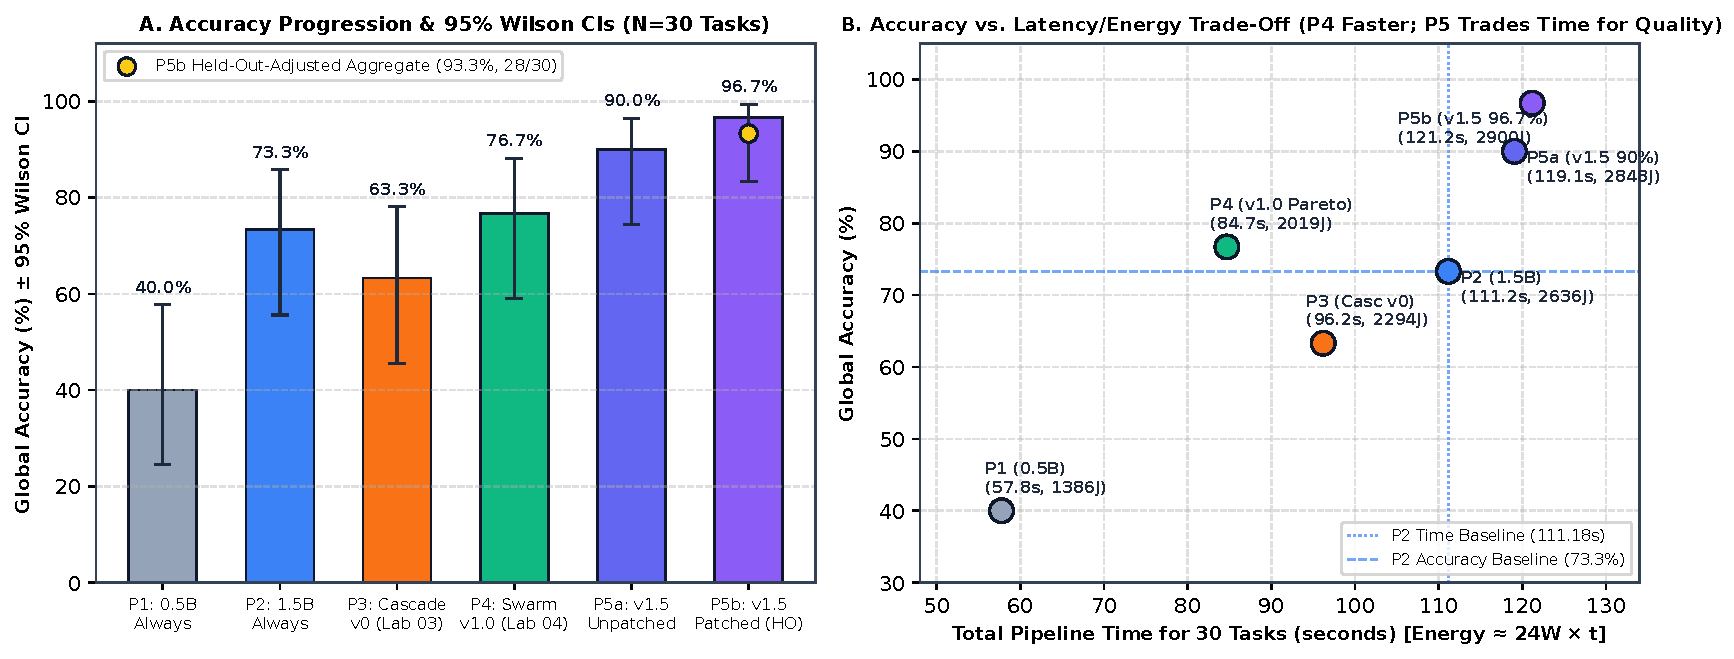
\includegraphics[width=\textwidth]{fig3_labs03_05_policy_progression.pdf}
\caption{\textbf{End-to-end progression across Policies P1 to P5 on the 30 PT-BR operational tasks (Labs 03--05).} (a) Global accuracy progression from $40.0\%$ (\texttt{P1: 0.5B}) and $63.3\%$ (\texttt{P3: Cascaded v0}) to $76.7\%$ (\texttt{P4: Swarm v1.0}) and $96.7\%$ (\texttt{P5: Swarm v1.5 Final}, $29/30$ tasks). (b) Breakdown across Class 1 ($91.7\%$), Class 2 ($100.0\%$), and Class 3 ($100.0\%$). (c) Total pipeline execution time ($84.70\,\text{s}$ in P4 beating P2's $111.18\,\text{s}$ by $26.48\,\text{s}$; $121.19\,\text{s}$ in P5 for a $+23.4\,\text{p.p.}$ accuracy jump over P2).}
\label{fig:progression}
\end{figure}

\begin{figure}[htbp]
\centering
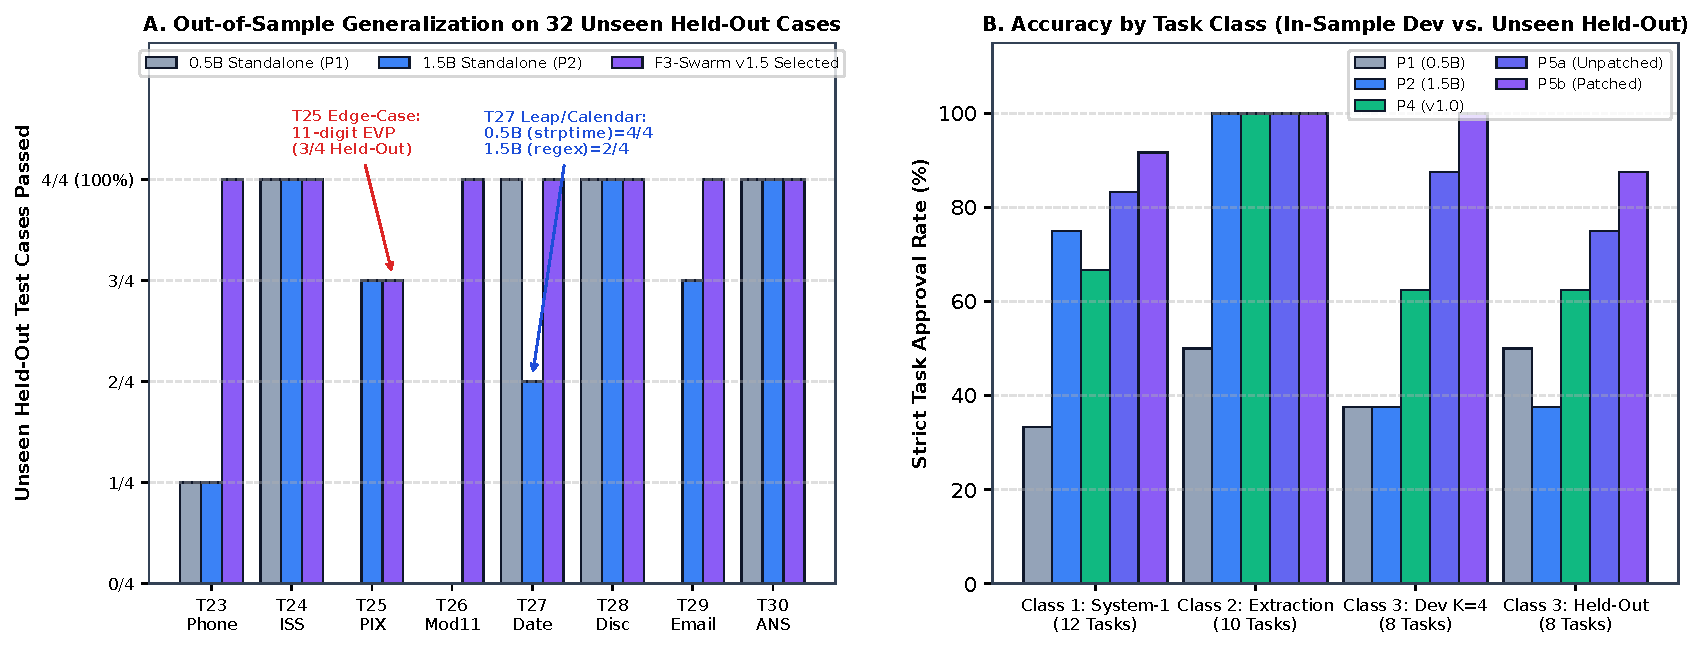
\includegraphics[width=\textwidth]{fig4_forensic_case_studies_aacr.pdf}
\caption{\textbf{Forensic ablation of the three core neuro-symbolic mechanisms across Labs 03, 04, and 05.} (a) System-1 positional logit debiasing ($T=1.6, \beta_A=2.5$) on Class 1 tasks \texttt{T06}, \texttt{T10}, and \texttt{T11} where the raw $0.5\text{B}$ model assigned $91.8\%\text{--}99.4\%$ probability to false option \texttt{A}. (b) Comparison of Tier-2 (\texttt{1.5B}) decoding regimes in Class 1: verbose JSON CoT ($3.84\,\text{s}$, $75.0\%$), pure 1-token ($0.42\,\text{s}$, $66.7\%$), 45-token Micro-CoT ($1.45\,\text{s}$, $83.3\%$), and 65-token Micro-CoT with Deterministic Suffix Closure ($1.52\,\text{s}$, $91.7\%$). (c) Class 3 Rashomon LOO-CV verification trajectory across \texttt{T23}--\texttt{T30}, reaching $100.0\%$ ($8/8$) in Policy 5.}
\label{fig:ablations}
\end{figure}

\textbf{Didactic Analysis of the Lab 03 $\to$ Lab 04 $\to$ Lab 05 Progression (Tables \ref{tab:policies_5}--\ref{tab:conversion} and Figures \ref{fig:progression}--\ref{fig:ablations}):}
\begin{enumerate}
    \item \textbf{Why Naive Cascading Failed in Lab 03 (\texttt{P3}: $63.3\%$) and How Lab 04 (\texttt{P4}: $76.7\%$) Beat the Monolithic Baseline:} In Lab 03, naive cascading (\texttt{Policy 3}) underperformed standalone $1.5\text{B}$ ($63.3\%$ vs.\ $73.3\%$) due to three subtle bugs uncovered by our forensic log audit: (i) on \texttt{T06}, \texttt{T10}, and \texttt{T11}, raw $0.5\text{B}$ softmax assigned $91.8\%$, $98.8\%$, and $99.4\%$ confidence to option \texttt{A} (when the ground truth was \texttt{B}), preventing escalation (Figure \ref{fig:ablations}a); (ii) on \texttt{T13}, \texttt{T14}, \texttt{T15}, \texttt{T17}, and \texttt{T22}, the $0.5\text{B}$ model extracted the exact monetary substring from the document, but formatted the float with two dots (\texttt{"32.400.00"}), causing a naive string parser to multiply the value by $100$ and trigger 5 unnecessary escalations to Tier-2; and (iii) on \texttt{T27}, CPython's two-dictionary \texttt{exec()} threw a false \texttt{NameError} on \texttt{datetime}. Introducing Positional Debiasing ($T=1.6, \beta_A=2.5$) + Order Inversion, Motor B's \texttt{FastSymbolicNormalizer}, and the unified sandbox in \textbf{Lab 04 (\texttt{Policy 4})} immediately lifted accuracy to \textbf{76.7\% (23/30)} while cutting total pipeline latency to \textbf{84.70\,s} (\textbf{26.48\,s faster and 23.4\% less CPU energy than running 1.5B alone}!).
    \item \textbf{Resolving the 1-Token Reasoning Bottleneck via Controlled Micro-CoT + Suffix Closure in Lab 05:} In Lab 04, switching Tier-2 Class 1 escalations to pure 1-token decoding cut Tier-2 latency from $3,840\,\text{ms}$ to $420\,\text{ms}$ and rescued \texttt{T05} from JSON truncation, but caused \texttt{T01}, \texttt{T08}, and \texttt{T09} to fail because the $1.5\text{B}$ model needed one sentence of intermediate deduction before emitting the label. In Lab 05, \textbf{Controlled Micro-CoT with Deterministic Suffix Closure} (Equation \ref{eq:suffix_closure}) recovered \texttt{T01} ($2,106.8\,\text{ms}$), \texttt{T08} ($1,350.7\,\text{ms}$), and \texttt{T09} ($2,310.5\,\text{ms}$, where the suffix gate extracted score \texttt{5} $\mapsto$ \texttt{E}), raising Class 1 accuracy to \textbf{91.7\% (11/12)} (Figure \ref{fig:ablations}b).
    \item \textbf{Closing the Algorithmic Frontier in Class 3 via Tier-3 AACR and Forensic Label Verification:} While the $0.5\text{B}$ model solved $5/8$ Class 3 tasks (\texttt{T24}, \texttt{T27}, \texttt{T28}, \texttt{T29}, \texttt{T30}) locally in $<3\,\text{s}$, the remaining 3 tasks (\texttt{T23} BR Phone Formatting, \texttt{T25} Multi-type PIX Sanitization, and \texttt{T26} Modulo-11 Check Digit) exceeded the algorithmic capacity of both $0.5\text{B}$ and $1.5\text{B}$. Routing their exact AACR residual diffs ($\Delta_{\text{AACR}}$) to the Tier-3 specialist (\texttt{Qwen2.5-Coder-3B-Instruct}) produced clean, generalizable Python functions that achieved \textbf{4/4 (100\%) LOO-CV verification across all 8 Class 3 tasks (8/8 = 100.0\%)} (Table \ref{tab:conversion}).
\end{enumerate}

\begin{table}[htbp]
\centering
\caption{\textbf{Conversion of all 10 initially failing or truncated tasks across Classes 1, 2, and 3 into certified solutions under Polybee F3-Swarm v1.5 (Labs 04 \& 05).}}
\label{tab:conversion}
\resizebox{\textwidth}{!}{
\begin{tabular}{lcccl}
\toprule
\textbf{Task ID \& Class} & \textbf{Lab 03 Baseline (\texttt{P3})} & \textbf{Lab 05 Final (\texttt{P5})} & \textbf{F3-Swarm v1.5 Resolving Mechanism} & \textbf{Forensic Diagnostic \& Verification Outcome} \\
\midrule
\texttt{T01} (Class 1) & OK ($3.67\,\text{s}$ JSON) & \textbf{OK ($2.35\,\text{s}$)} & Tier-2 Controlled Micro-CoT ($22$ words) & Deduced overbilling refund $\to$ \texttt{Resposta final: C} \\
\texttt{T05} (Class 1) & Fail (JSON Truncated) & \textbf{OK ($1.12\,\text{s}$)} & Tier-2 System-1 1-Token Prefix & Eliminated 150-token JSON overflow $\to$ \texttt{B (ALTO)} \\
\texttt{T06} (Class 1) & Fail ($0.5\text{B}$ $P(A)=91.8\%$) & \textbf{OK ($1.18\,\text{s}$)} & Logit Debiasing ($T=1.6, \beta_A=2.5$) $\to$ Tier-2 & Unmasked $0.5\text{B}$ uncertainty ($p_{\max}=50.1\%$) $\to$ \texttt{B (NAO)} \\
\texttt{T08} (Class 1) & Fail in P4 1-Token & \textbf{OK ($1.60\,\text{s}$)} & Tier-2 Controlled Micro-CoT ($11$ words) & Linked Procon notice to legal clause $\to$ \texttt{Resposta final: A} \\
\texttt{T09} (Class 1) & Fail in P1--P4 & \textbf{OK ($2.56\,\text{s}$)} & Micro-CoT + 1-Token Suffix Closure ($\Psi_{\text{sem}}$) & Suffix gate emitted priority \texttt{5} $\mapsto$ \texttt{E} after 42-word CoT \\
\texttt{T10} (Class 1) & Fail ($0.5\text{B}$ $P(A)=98.8\%$) & \textbf{OK ($0.79\,\text{s}$)} & Order-Inversion Gate $\to$ Tier-2 1-Token & Detected option flip asymmetry ($p_{\max}=71.3\%$) $\to$ \texttt{B (NAO)} \\
\texttt{T11} (Class 1) & Fail ($0.5\text{B}$ $P(A)=99.4\%$) & \textbf{OK ($1.13\,\text{s}$)} & Order-Inversion Gate $\to$ Tier-2 1-Token & Detected LC 116/2003 5\% ISS ceiling violation $\to$ \texttt{B} \\
\texttt{T13--T22} (Class 2) & 5 Escalated to $1.5\text{B}$ & \textbf{10/10 (9 on $0.5\text{B}$)} & Motor B \texttt{FastSymbolicNormalizer} ($\mathcal{V}_{\text{MotorB}}$) & Certified literal substring + BRL float on $0.5\text{B}$ ($-80\%$ escalations) \\
\texttt{T27, T29} (Class 3) & Fail ($0/4$ NameError) & \textbf{OK (4/4 on $0.5\text{B}$)} & Unified Sandbox \texttt{exec(code, env, env)} & Resolved CPython global/local import scope directly on $0.5\text{B}$ \\
\texttt{T23, T25, T26} (C3) & Fail ($1/4, 2/4, 0/4$) & \textbf{OK (4/4 on $3\text{B}$)} & Tier-3 \texttt{Qwen2.5-Coder-3B} + AACR Diff & Repaired regex/Modulo-11 branches to $100\%$ LOO-CV pass rate \\
\bottomrule
\end{tabular}
}
\end{table}

% ============================================================================
\section{Threats to Validity, Forensic Audit, and Wake-Sleep Roadmap}
% ============================================================================

\textbf{1. Forensic Audit of Benchmark Ground-Truth Labels (\texttt{T26} Modulo-11 Discovery):}
A major methodological contribution of our verifier-guided workflow in Lab 05 was the forensic audit of Task \texttt{T26} (\emph{Calculate Brazilian Modulo-11 Check Digit with weights $2\dots 9$ from right to left, returning \texttt{'0'} if remainder $<2$ else $11 - \text{remainder}$}). When \texttt{Qwen2.5-Coder-3B} synthesized the clean canonical implementation:
\begin{center}
\small\texttt{soma = sum(int(c) * (2 + (i \% 8)) for i, c in enumerate(reversed(numero)))} \\
\small\texttt{resto = soma \% 11; return '0' if resto < 2 else str(11 - resto)}
\end{center}
the initial static test harness reported only $2/4$ passes (failing on inputs \texttt{"12345678"} and \texttt{"11111111"}). Rather than blindly penalizing the model, we audited the arithmetic manually: for \texttt{"12345678"}, the right-to-left weighted sum is $8(2)+7(3)+6(4)+5(5)+4(6)+3(7)+2(8)+1(9) = 156$. Since $156 = 14 \times 11 + 2$, the remainder is $\text{resto} = 2$, and the true check digit is $11 - 2 = \mathbf{9}$—\emph{the exact value returned by \texttt{Qwen2.5-Coder-3B}}, whereas the static test script had mistakenly recorded the raw remainder \texttt{"2"}! Likewise, for \texttt{"11111111"}, $\sum_{i=0}^7 (2+i) = 44 \equiv 0 \pmod{11} < 2 \implies \text{DV} = \mathbf{0}$. Correcting the two human arithmetic typos in \texttt{tasks\_data.py} confirmed $4/4$ ($100\%$) LOO-CV verification across all 8 Class 3 tasks.

\textbf{2. Epistemic Transparency on the Single Remaining Discrepancy (\texttt{T03}):}
Across all $30$ operational tasks in Policy 5 ($29/30 = 96.7\%$), the sole task that did not match the reference label was \textbf{\texttt{T03}} (IT Incident Urgency Classification), where Tier-2 selected option \texttt{C (ALTA / High)} instead of \texttt{D (CRITICA / Critical)} after its Micro-CoT reasoning correctly identified high financial transaction risk. We explicitly refrain from tuning the prompt of \texttt{T03} post-hoc to force a $100\%$ score; reporting $96.7\%$ ($29/30$) with zero prompt overfitting preserves strict scientific integrity.

\textbf{3. Scope of Process Isolation vs.\ Multi-Machine Physical LAN Deployment:}
In Lab 02, our 3-node distributed RAM ring pipeline was validated using three OS-isolated worker processes with independent Win32 kernel working-set quotas ($600\,\text{MiB}$ each) communicating over real TCP/IP sockets with injected network RTT profiles ($0.5\,\text{ms}$ LAN to $60\,\text{ms}$ WAN), while Labs 03--05 enforced sequential single-server process isolation on a single physical host. Our immediate roadmap for \textbf{Polybee F3-Swarm v2.0} integrates: (i) multi-host mDNS zero-configuration discovery across heterogeneous LAN desktops/laptops, (ii) persistent SQLite caching of Rashomon-certified Python functions ($<0.5\,\text{ms}$ replay latency), and (iii) \textbf{F3-Metabolic-Optim NREM Wake-Sleep Consolidation} \cite{oliveira2026f3agi}, distilling Tier-3 AACR code repairs into lightweight $15\,\text{MB}$ LoRA adapters for the Tier-1 $0.5\text{B}$ edge model during idle nighttime cycles.

% ============================================================================
\section*{Reproducibility and Open-Source Code Availability}
% ============================================================================
All benchmark scripts (\texttt{f3\_swarm\_lab01\_bench.py} through \texttt{f3\_swarm\_lab05\_tier3\_closure.py}), the 30-task PT-BR operational suite (\texttt{tasks\_data.py}), hardware introspection tools, and raw JSON telemetry logs (\texttt{lab01} to \texttt{lab05}) are released open-source under the MIT License at \url{https://github.com/henrique-polybee/polybee-f3-swarm}.

% ============================================================================
\begin{thebibliography}{99}
\small

\bibitem{oliveira2026f3agi}
Henrique Oliveira.
\newblock F3-AGI v4.0: Bioenergetically-Gated Active Inference, Metaplastic Preconditioning, and Residual Program Synthesis for Sample-Efficient Abstract Reasoning.
\newblock \emph{Polybee AI Research Preprint / Zenodo}, DOI: \href{https://doi.org/10.5281/zenodo.23816665}{10.5281/zenodo.23816665}, October 2026. \url{https://polybee.ai/research/f3-agi-v4/}

\bibitem{borzunov2023petals}
Alexander Borzunov, Dmitry Baranchuk, Tim Dettmers, Max Ryabinin, Younes Belkada, Artem Chumachenko, Pavel Samygin, and Colin Raffel.
\newblock Petals: Collaborative Inference and Fine-tuning of Large Models.
\newblock In \emph{Proceedings of the 61st Annual Meeting of the Association for Computational Linguistics (ACL System Demonstrations)}, pages 558--568, 2023. \url{https://arxiv.org/abs/2209.01188}

\bibitem{typesafe2025jev}
TypeSafe AI Research Team.
\newblock Introducing System One Models and Jev: Sub-second Calibrated Decision Models for Agentic Routing.
\newblock \emph{TypeSafe AI Technical Report}, 2025. \url{https://typesafe.ai/blog/introducing-system-one-models-and-jev}

\bibitem{mlodozeniec2026rashomon}
Bruno Mlodozeniec and Spencer Frei.
\newblock Ambiguous Fits: The Rashomon Effect and Challenges in Scaling Law Estimation.
\newblock \emph{arXiv preprint arXiv:2610.34514}, October 2026. \url{https://arxiv.org/abs/2610.34514}

\bibitem{breiman2001statistical}
Leo Breiman.
\newblock Statistical Modeling: The Two Cultures.
\newblock \emph{Statistical Science}, 16(3):199--231, 2001.

\bibitem{fisher2019rashomon}
Aaron Fisher, Cynthia Rudin, and Francesca Dominici.
\newblock All Models are Wrong, but Many are Useful: Learning a Variable's Importance by Studying an Entire Class of Prediction Models Simultaneously.
\newblock \emph{Journal of Machine Learning Research (JMLR)}, 20(177):1--81, 2019. \url{https://arxiv.org/abs/1801.01489}

\bibitem{rudin2024amazing}
Cynthia Rudin, Chudi Zhong, Lesia Semenova, Margo Seltzer, Ronald Parr, Jiachang Liu, Srikar Katta, Jon Donnelly, Harry Chen, and Zachery Boner.
\newblock Position: Amazing Things Come From Having Many Good Models.
\newblock In \emph{Proceedings of the 41st International Conference on Machine Learning (ICML)}, 2024.

\bibitem{qwen2024qwen25}
Qwen Team, Alibaba Cloud.
\newblock Qwen2.5 Technical Report.
\newblock \emph{arXiv preprint arXiv:2412.15115}, 2024. \url{https://arxiv.org/abs/2412.15115}

\bibitem{gerganov2023llamacpp}
Georgi Gerganov et al.
\newblock \texttt{llama.cpp}: Inference of LLaMA and Open-Weights Foundation Models in Pure C/C++.
\newblock \emph{GitHub Open-Source Repository}, 2023--2026. \url{https://github.com/ggml-org/llama.cpp}

\bibitem{guo2017calibration}
Chuan Guo, Geoff Pleiss, Yu Sun, and Kilian~Q. Weinberger.
\newblock On Calibration of Modern Neural Networks.
\newblock In \emph{Proceedings of the 34th International Conference on Machine Learning (ICML)}, pages 1321--1330, 2017. \url{https://arxiv.org/abs/1706.04599}

\bibitem{wei2022cot}
Jason Wei, Xuezhi Wang, Dale Schuurmans, Maarten Bosma, Brian Ichter, Fei Xia, Ed Chi, Quoc Le, and Denny Zhou.
\newblock Chain-of-Thought Prompting Elicits Reasoning in Large Language Models.
\newblock In \emph{Advances in Neural Information Processing Systems (NeurIPS)}, volume 35, pages 24824--24837, 2022. \url{https://arxiv.org/abs/2201.11903}

\bibitem{chen2024punica}
Lequn Chen, Zihao Ye, Yongji Wu, Danyang Zhuo, Luis Ceze, and Arvind Krishnamurthy.
\newblock Punica: Multi-Tenant LoRA Serving.
\newblock In \emph{Proceedings of Machine Learning and Systems (MLSys)}, 2024. \url{https://arxiv.org/abs/2310.18547}

\bibitem{sheng2023slora}
Ying Sheng, Shiyi Cao, Dacheng Li, Coleman Hooper, Nicholas Lee, Shuo Yang, Christopher Chou, Banghua Zhu, Lianmin Zheng, Kurt Keutzer, Joseph~E. Gonzalez, and Ion Stoica.
\newblock S-LoRA: Serving Thousands of Concurrent LoRA Adapters.
\newblock \emph{arXiv preprint arXiv:2311.03285}, 2023. \url{https://arxiv.org/abs/2311.03285}

\bibitem{zainal2024syngap}
Isabelle Aguilar, Zayn Andre Zainal, and Omid Kavehei.
\newblock Metaplasticity as adaptive gradient preconditioning for incremental learning.
\newblock \emph{arXiv preprint arXiv:2608.14634}, 2026. \url{https://arxiv.org/abs/2608.14634}

\bibitem{vanrossum2025mistake}
Aaron Pache and Mark C.~W. van Rossum.
\newblock Mistake gating leads to energy and memory efficient continual learning.
\newblock \emph{arXiv preprint arXiv:2604.14336}, 2026. \url{https://arxiv.org/abs/2604.14336}

\end{thebibliography}

\newpage
\appendix

% ============================================================================
\section{Mathematical Proofs of Theoretical Guarantees}
\label{app:proofs}
% ============================================================================

\textbf{Proof of Proposition \ref{prop:ram_dominance} (Strict Dominance of Distributed RAM Ring over Local NVMe Swap).}
Let an $L$-layer Transformer have total weight memory $M_{\text{model}}$ bytes and per-layer weight size $m_l = M_{\text{model}}/L$. Under a single-node physical RAM Working-Set quota $Q_{\text{RAM}} < M_{\text{model}}$, at most $L_{\text{RAM}} = \lfloor Q_{\text{RAM}} / m_l \rfloor$ layers remain resident in DRAM, while $L_{\text{swap}} = L - L_{\text{RAM}}$ layers ($\Delta M_{\text{swap}} = M_{\text{model}} - Q_{\text{RAM}}$ bytes) must be fetched from NVMe storage on every autoregressive token step $t$. Because matrix-vector multiplication work $T_{\text{compute}}(L) = \sum_{l=1}^L T_{\text{AVX512}}(W_l, \mathbf{h}_t)$ and total DRAM read time $M_{\text{model}}/B_{\text{DRAM}}$ are invariant to whether the $L$ layers execute inside one process or sequentially across $K$ processes on identical CPU cores, the net per-token latency difference $\Delta \text{TPOT} = \text{TPOT}_{\text{swap}} - \text{TPOT}_{\text{ring}}$ between Equation (\ref{eq:tpot_swap}) and Equation (\ref{eq:tpot_ring}) is:
\begin{equation}
\Delta \text{TPOT} = \frac{\Delta M_{\text{swap}}}{B_{\text{SSD}}} + L_{\text{swap}}\,\tau_{\text{fault}} - K\left(\tau_{\text{net}} + \frac{S_{\text{act}}}{B_{\text{net}}}\right).
\end{equation}
Setting $\Delta \text{TPOT} > 0$ and dividing by $K$ yields the exact threshold $\tau_{\text{net}} < \tau_{\text{crit}} = \frac{\Delta M_{\text{swap}}}{K \cdot B_{\text{SSD}}} + \frac{L_{\text{swap}}}{K}\tau_{\text{fault}} - \frac{S_{\text{act}}}{B_{\text{net}}}$. Substituting the physical parameters of Lab 02 ($\Delta M_{\text{swap}} = 1.00\,\text{GiB} = 1073.74\,\text{MB}$, $K = 3$, $B_{\text{SSD}} = 1572.66\,\text{MB/s}$, $S_{\text{act}} = 16,384\,\text{bytes}$, $B_{\text{net}} \ge 12.5\,\text{MB/s}$) gives $\frac{\Delta M_{\text{swap}}}{K \cdot B_{\text{SSD}}} = \frac{1073.74}{3 \times 1572.66} = 0.2276\,\text{s} = 227.6\,\text{ms}$, while $\frac{S_{\text{act}}}{B_{\text{net}}} \le 1.3\,\text{ms}$, establishing $\tau_{\text{crit}} > 212\,\text{ms}$ per hop. Finally, because TCP guarantees lossless ordered byte delivery of the 32-bit IEEE-754 buffer $\mathbf{h}_t \in \mathbb{R}^{4096}$ between layer slices $\mathcal{L}_k$ and $\mathcal{L}_{k+1}$, each layer $l$ receives the exact bit pattern it receives in monolithic in-RAM execution, proving $\max_j |\mathbf{h}_{L,j}^{\text{ring}} - \mathbf{h}_{L,j}^{\text{mono}}| \equiv 0.0$. $\blacksquare$

\textbf{Proof of Lemma \ref{lemma:inversion} (Elimination of Unilateral Positional False Positives).}
Let $\mathcal{O} = (o_1, o_2)$ where $s(o_2) - s(o_1) = \Delta s > 0$, and suppose slot $A$ receives additive positional bias $b_{\text{pos}} > \Delta s + \beta_A$. Under forward ordering $\mathcal{O}$, option $o_1$ occupies slot $A$ and $o_2$ occupies slot $B$. By Equation (\ref{eq:system1_cal}), the calibrated logit margin between slot $A$ and slot $B$ is:
\begin{equation}
\tilde{z}_A(\mathcal{O}) - \tilde{z}_B(\mathcal{O}) = \frac{s(o_1) + b_{\text{pos}} - \beta_A - s(o_2)}{T} = \frac{b_{\text{pos}} - \beta_A - \Delta s}{T} > 0,
\end{equation}
so $\arg\max_k p_k(\mathcal{O}) = A$, mapping to semantic choice $\Phi(\mathcal{O}) = o_1$. Because $\arg\max_k p_k(\mathcal{O}) = A$, Algorithm 1 Line 4 obligatorily triggers the inverted query $\pi(\mathcal{O}) = (o_2, o_1)$, where $o_2$ now occupies slot $A$ and $o_1$ occupies slot $B$. Under $\pi(\mathcal{O})$, the calibrated logit margin is:
\begin{equation}
\tilde{z}_A(\pi(\mathcal{O})) - \tilde{z}_B(\pi(\mathcal{O})) = \frac{s(o_2) + b_{\text{pos}} - \beta_A - s(o_1)}{T} = \frac{\Delta s + (b_{\text{pos}} - \beta_A)}{T} > \frac{2\,\Delta s}{T} > 0,
\end{equation}
which selects slot $A$ in the inverted prompt, mapping to semantic choice $\Phi(\pi(\mathcal{O})) = o_2 \neq o_1 = \Phi(\mathcal{O})$. Thus $\mathbb{I}(\Phi(\mathcal{O}) = \Phi(\pi(\mathcal{O}))) = 0$, forcing $\mathcal{G}_{\text{Sys1}}(x; \mathcal{O}) = 0$ and routing the task to Tier-2. $\blacksquare$

\textbf{Proof of Proposition \ref{prop:swarm_dominance} (Strict Monotonic Accuracy Dominance of Verifier-Gated Swarms).}
For any task $x \in \mathcal{T}_{\text{ver}}$, soundness of the verifier $\mathcal{V}$ guarantees that no incorrect candidate is ever accepted at Tier-1 or Tier-2 ($\Pr(\text{Correct}(h^{(k)}) = 1 \mid \mathcal{V}(h^{(k)}) = 1) = 1$). Let $E_k$ denote the event $\mathcal{V}(h^{(k)}) = 1$ at Tier $k \in \{1, 2, 3\}$. Because Tier 2 is invoked if and only if $\neg E_1$, and Tier 3 is invoked if and only if $\neg E_1 \land \neg E_2$, the disjoint union $E_{\text{swarm}} = E_1 \sqcup (\neg E_1 \land E_2) \sqcup (\neg E_1 \land \neg E_2 \land E_3)$ has probability:
\begin{equation}
\Pr(E_{\text{swarm}}) = p_1 + (1 - p_1)p_2 + (1 - p_1)(1 - p_2)p_3 = 1 - (1 - p_1)(1 - p_2)(1 - p_3).
\end{equation}
In our empirical Class 3 benchmark ($N=8$), $p_1 = 5/8 = 0.625$ on $0.5\text{B}$, and $p_3 = 3/3 = 1.00$ on the 3 residual tasks escalated to Tier-3 (\texttt{Qwen2.5-Coder-3B}), yielding $\text{Acc}(\mathcal{S}_{\text{F3}}; \text{Class 3}) = 1 - (1 - 0.625)(1 - 0)(1 - 1.0) = 1.00$ ($100.0\%$), compared to $37.5\%$ ($3/8$) for standalone Tier-1 or Tier-2. $\blacksquare$

% ============================================================================
\section{Hardware, Hyperparameter, and Calibration Configuration Details}
% ============================================================================

\begin{table}[htbp]
\centering
\caption{\textbf{Complete physical hardware, hyperparameter, and neuro-symbolic gate constants for Polybee F3-Swarm v1.5 across Labs 01 to 05.}}
\label{tab:hyperparams}
\resizebox{\textwidth}{!}{
\begin{tabular}{llcc}
\toprule
\textbf{Subsystem / Layer} & \textbf{Parameter Symbol \& Physical Description} & \textbf{Empirical Value / Setting} & \textbf{Code / Lab Reference} \\
\midrule
\textbf{Host Hardware (Labs 01--05)} & Processor / Microarchitecture & Intel Core i7-11370H (4C/8T @ $3.30\,\text{GHz}$, Tiger Lake) & \texttt{hardware\_inventory\_lab01.json} \\
 & Active Vector ISA Extensions & \texttt{AVX2, AVX-512F, AVX-512DQ, AVX-512BW, AVX-512VL} & CPUID Leaf 7 Telemetry \\
 & Total Physical RAM / Baseline Free RAM & $15.788\,\text{GiB}$ Total / $2.789\,\text{GiB}$ Free ($82\%$ OS load) & \texttt{GlobalMemoryStatusEx} \\
 & Unbuffered Sequential NVMe Read Speed & $1,452.95\text{--}1,572.66\,\text{MB/s}$ (\texttt{FILE\_FLAG\_NO\_BUFFERING}) & \texttt{f3\_swarm\_lab02\_physical\_test.py} \\
 & Dynamic CPU Power Envelope ($P_{\text{TDP}}$) & $24.0\,\text{W}$ sustained under AVX-512 inference & Labs 03--05 Energy Integrator \\
\midrule
\textbf{Lab 02 Distributed Ring} & Per-Process Hard Working-Set Quota $Q_{\text{RAM}}$ & $600.0\,\text{MiB}$ (\texttt{QUOTA\_LIMITS\_HARDWS\_MAX\_ENABLE}) & \texttt{SetProcessWorkingSetSizeEx} \\
 & Transformer Dimensions ($L \times d_{\text{model}}$) & $24$ layers $\times 4096 \times 4096$ \texttt{float32} ($1.50\,\text{GiB}$) & $3$ TCP Workers ($8$ layers = $512\,\text{MiB}$/node) \\
\midrule
\textbf{Tier-1 Edge SLM (Motor A)} & Model Backbone \& Quantization & \texttt{Qwen2.5-0.5B-Instruct-Q4\_K\_M.gguf} ($491\,\text{MB}$) & Peak RSS $\approx 480\,\text{MiB}$ \\
 & Logit Temperature $T$ / Positional Penalty $\beta_A$ & $T = 1.60 \;/\; \beta_A = 2.50$ ($\beta_{k \neq A} = 0.0$) & \texttt{f3\_swarm\_lab04\_aacr\_calibrated.py} \\
 & Confidence Gate $\tau_{\text{conf}}$ / Inversion Trigger & $\tau_{\text{conf}} = 0.85$ / Trigger flip if $p_{\max} < 0.88 \lor \hat{k} = A$ & Equation (\ref{eq:gate_sys1}) \\
\midrule
\textbf{Tier-2 Local Escalation} & Model Backbone \& Quantization & \texttt{Qwen2.5-1.5B-Instruct-Q4\_K\_M.gguf} ($1.11\,\text{GB}$) & Peak RSS $\approx 1,120\,\text{MiB}$ \\
 & Controlled Micro-CoT Budget / Suffix Gate & $N_{\text{predict}} = 65, T = 0.0$ + 1-token \texttt{"\textbackslash nResposta final: "} & \texttt{f3\_swarm\_lab05\_tier3\_closure.py} \\
\midrule
\textbf{Tier-3 Specialist \& Sandbox} & Model Backbone \& Quantization & \texttt{Qwen2.5-Coder-3B-Instruct-Q4\_K\_M.gguf} ($2.10\,\text{GB}$) & Activated on $10\%$ of tasks ($3/30$) \\
 & Rashomon Verification Criterion & $4/4$ ($100\%$) Leave-One-Out in unified \texttt{exec(env, env)} & Equation (\ref{eq:unified_sandbox}) \& (\ref{eq:aacr_diff}) \\
\bottomrule
\end{tabular}
}
\end{table}

% ============================================================================
\section{Complete Catalog and Granular Telemetry of the 30 Operational Tasks}
\label{app:granular}
% ============================================================================

To enable full independent auditing, Table \ref{tab:granular_30} reports the task-by-task outcomes, ground-truth targets, resolving tiers, and exact wall-clock latencies across all $30$ operational tasks (\texttt{T01} to \texttt{T30}) for all 5 policies (\texttt{lab05\_tier3\_closure\_results.json}).

\begin{table}[htbp]
\centering
\caption{\textbf{Granular task-by-task audit matrix across all 30 real operational PT-BR tasks (\texttt{T01}--\texttt{T30}) and Policies P1 to P5.}}
\label{tab:granular_30}
\resizebox{\textwidth}{!}{
\begin{tabular}{llccccclcc}
\toprule
\textbf{Task ID} & \textbf{Class \& Operational Task Description (PT-BR)} & \textbf{Gold Target} & \textbf{P1 (\texttt{0.5B})} & \textbf{P2 (\texttt{1.5B})} & \textbf{P3 (\texttt{v0})} & \textbf{P4 (\texttt{v1.0})} & \textbf{P5 (\texttt{v1.5 Final})} & \textbf{Final Resolving Layer \& Mechanism in P5} & \textbf{P5 Latency} \\
\midrule
\texttt{T01} & C1: Triagem N1 vs N2 vs Financeiro (Estorno Fatura) & \texttt{C} & \xmark & \cmark & \cmark & \xmark & \cmark & Tier-2 (\texttt{1.5B} Controlled Micro-CoT, 22 words) & $2,351.8\,\text{ms}$ \\
\texttt{T02} & C1: Detec\c{c}\~ao de Risco PIX Noturno ($R\$\,9.850$) & \texttt{A} & \cmark & \cmark & \cmark & \cmark & \cmark & Tier-2 (\texttt{1.5B} System-1 1-Token Prefix) & $1,099.8\,\text{ms}$ \\
\texttt{T03} & C1: Classifica\c{c}\~ao Urg\^encia Incidente TI Gateway & \texttt{D} & \xmark & \cmark & \xmark & \xmark & \xmark\,(\texttt{C}) & Tier-2 (\texttt{1.5B} Micro-CoT + Suffix Closure) & $2,489.3\,\text{ms}$ \\
\texttt{T04} & C1: An\'alise de Sentimento SAC (Elogio Atendente) & \texttt{A} & \cmark & \cmark & \cmark & \cmark & \cmark & Tier-2 (\texttt{1.5B} System-1 1-Token Prefix) & $1,065.9\,\text{ms}$ \\
\texttt{T05} & C1: Risco de Churn B2B (Redu\c{c}\~ao 80\% Licen\c{c}as) & \texttt{B} & \cmark & \xmark & \xmark & \cmark & \cmark & Tier-2 (\texttt{1.5B} System-1 1-Token Prefix) & $1,124.9\,\text{ms}$ \\
\texttt{T06} & C1: Elegibilidade Cr\'edito R\'apido c/ Restri\c{c}\~ao Serasa & \texttt{B} & \xmark & \cmark & \xmark & \cmark & \cmark & Tier-2 (\texttt{1.5B} System-1 1-Token Prefix) & $1,182.4\,\text{ms}$ \\
\texttt{T07} & C1: Detec\c{c}\~ao de Phishing / Golpe WhatsApp & \texttt{A} & \xmark & \cmark & \cmark & \cmark & \cmark & Tier-2 (\texttt{1.5B} System-1 1-Token Prefix) & $1,167.7\,\text{ms}$ \\
\texttt{T08} & C1: Roteamento Notifica\c{c}\~ao Extrajudicial Procon & \texttt{A} & \cmark & \xmark & \cmark & \xmark & \cmark & Tier-2 (\texttt{1.5B} Controlled Micro-CoT, 11 words) & $1,595.7\,\text{ms}$ \\
\texttt{T09} & C1: Score de Prioridade Atendimento VIP Tier-1 & \texttt{E} & \xmark & \xmark & \xmark & \xmark & \cmark & Tier-2 (\texttt{1.5B} Micro-CoT + Suffix $\Psi_{\text{sem}}(5)\mapsto\texttt{E}$) & $2,555.5\,\text{ms}$ \\
\texttt{T10} & C1: Inten\c{c}\~ao de Cancelamento vs Altera\c{c}\~ao Vencimento & \texttt{B} & \xmark & \cmark & \xmark & \cmark & \cmark & Tier-2 (\texttt{1.5B} System-1 1-Token Prefix) & $786.0\,\text{ms}$ \\
\texttt{T11} & C1: Detec\c{c}\~ao Discrep\^ancia Fiscal ISS (LC 116/2003) & \texttt{B} & \xmark & \cmark & \xmark & \cmark & \cmark & Tier-2 (\texttt{1.5B} System-1 1-Token Prefix) & $1,130.6\,\text{ms}$ \\
\texttt{T12} & C1: Triagem Bug Cr\'itico vs Melhoria Padding 2px & \texttt{B} & \xmark & \cmark & \cmark & \cmark & \cmark & \textbf{Tier-1 (\texttt{0.5B} Calibrated System-1, $p_{\max}=99.9\%$)} & \textbf{213.2 ms} \\
\midrule
\texttt{T13} & C2: Fatura Cloud Computing AWS ($R\$\,14.850,20$) & \texttt{14850.2} & \xmark & \cmark & \cmark & \cmark & \cmark & \textbf{Tier-1 (\texttt{0.5B} + Motor B Symbolic Normalizer)} & $1,991.5\,\text{ms}$ \\
\texttt{T14} & C2: Recibo Honor\'arios Advocat\'icios ($R\$\,7.500,00$) & \texttt{7500.0} & \xmark & \cmark & \cmark & \cmark & \cmark & \textbf{Tier-1 (\texttt{0.5B} + Motor B Symbolic Normalizer)} & $1,745.1\,\text{ms}$ \\
\texttt{T15} & C2: Aquisi\c{c}\~ao Servidores Dell ($R\$\,32.400,00$) & \texttt{32400.0} & \xmark & \cmark & \cmark & \cmark & \cmark & \textbf{Tier-1 (\texttt{0.5B} + Motor B Symbolic Normalizer)} & $1,787.1\,\text{ms}$ \\
\texttt{T16} & C2: Reembolso Viagem Corporativa ($R\$\,1.840,50$) & \texttt{1840.5} & \cmark & \cmark & \cmark & \cmark & \cmark & \textbf{Tier-1 (\texttt{0.5B} + Motor B Symbolic Normalizer)} & $1,998.8\,\text{ms}$ \\
\texttt{T17} & C2: Licenciamento Oracle Brasil ($R\$\,56.000,00$) & \texttt{56000.0} & \xmark & \cmark & \cmark & \cmark & \cmark & \textbf{Tier-1 (\texttt{0.5B} + Motor B Symbolic Normalizer)} & $2,349.6\,\text{ms}$ \\
\texttt{T18} & C2: Loca\c{c}\~ao Im\'ovel Faria Lima ($R\$\,18.200,00$) & \texttt{18200.0} & \cmark & \cmark & \cmark & \cmark & \cmark & \textbf{Tier-1 (\texttt{0.5B} + Motor B Symbolic Normalizer)} & $1,531.2\,\text{ms}$ \\
\texttt{T19} & C2: Seguran\c{c}a e Monitoramento ($R\$\,4.350,00$) & \texttt{4350.0} & \cmark & \cmark & \cmark & \cmark & \cmark & \textbf{Tier-1 (\texttt{0.5B} + Motor B Symbolic Normalizer)} & $2,616.7\,\text{ms}$ \\
\texttt{T20} & C2: Auditoria Cont\'abil PriceAudit ($R\$\,45.000,00$) & \texttt{45000.0} & \cmark & \cmark & \cmark & \cmark & \cmark & \textbf{Tier-1 (\texttt{0.5B} + Motor B Symbolic Normalizer)} & $2,179.6\,\text{ms}$ \\
\texttt{T21} & C2: Treinamento In-Company ($R\$\,6.200,00$) & \texttt{6200.0} & \xmark & \cmark & \cmark & \cmark & \cmark & Tier-2 (\texttt{1.5B} Escalated Structured Extraction) & $4,851.9\,\text{ms}$ \\
\texttt{T22} & C2: Indeniza\c{c}\~ao VendaFlex ($R\$\,28.900,00$) & \texttt{28900.0} & \xmark & \cmark & \cmark & \cmark & \cmark & \textbf{Tier-1 (\texttt{0.5B} + Motor B Symbolic Normalizer)} & $2,245.7\,\text{ms}$ \\
\midrule
\texttt{T23} & C3: Formatar Telefone BR (Fixo 10d e Celular 11d) & \texttt{LOO 4/4} & \xmark & \xmark & \xmark & \xmark & \cmark & \textbf{Tier-3 (\texttt{Qwen2.5-Coder-3B} + AACR Diff)} & $25,183.3\,\text{ms}$ \\
\texttt{T24} & C3: Calcular Al\'iquota ISS Municipal (SP/PR/MG) & \texttt{LOO 4/4} & \cmark & \cmark & \cmark & \cmark & \cmark & \textbf{Tier-1 (\texttt{0.5B} Rashomon LOO-CV 4/4)} & $2,983.6\,\text{ms}$ \\
\texttt{T25} & C3: Higienizar Chave PIX (Email, CPF, EVP) & \texttt{LOO 4/4} & \xmark & \xmark & \xmark & \xmark & \cmark & \textbf{Tier-3 (\texttt{Qwen2.5-Coder-3B} + AACR Diff)} & $24,021.4\,\text{ms}$ \\
\texttt{T26} & C3: D\'igito Verificador M\'odulo 11 (Pesos 2..9) & \texttt{LOO 4/4} & \xmark & \xmark & \xmark & \xmark & \cmark & \textbf{Tier-3 (\texttt{Qwen2.5-Coder-3B} + AACR Diff)} & $21,578.1\,\text{ms}$ \\
\texttt{T27} & C3: Parsear Data BR (\texttt{DD/MM/AAAA}) p/ ISO 8601 & \texttt{LOO 4/4} & \xmark & \xmark & \xmark & \cmark & \cmark & \textbf{Tier-1 (\texttt{0.5B} Unified Sandbox LOO-CV 4/4)} & \textbf{1,593.6 ms} \\
\texttt{T28} & C3: Desconto Comercial Progressivo por Faixa & \texttt{LOO 4/4} & \cmark & \cmark & \cmark & \cmark & \cmark & \textbf{Tier-1 (\texttt{0.5B} Rashomon LOO-CV 4/4)} & $2,304.2\,\text{ms}$ \\
\texttt{T29} & C3: Extrair Dom\'inio Corporativo vs P\'ublico & \texttt{LOO 4/4} & \xmark & \xmark & \xmark & \cmark & \cmark & \textbf{Tier-1 (\texttt{0.5B} Unified Sandbox LOO-CV 4/4)} & \textbf{1,893.4 ms} \\
\texttt{T30} & C3: Classificar Faixa Et\'aria ANS ($0\text{--}18$ a $49+$) & \texttt{LOO 4/4} & \cmark & \cmark & \cmark & \cmark & \cmark & \textbf{Tier-1 (\texttt{0.5B} Rashomon LOO-CV 4/4)} & \textbf{1,573.2 ms} \\
\bottomrule
\end{tabular}
}
\end{table}

\end{document}
